{\justifying
	\chapterimage{jpg/LeonardoDaVinci.jpeg}{3cm}
	\chapter[Tecnologías para Cloud Computing]{Tecnologías Asociadas a Computación en la Nube}
	\epigraph{Simplicity is the ultimate sophistication.}{--- \textup{Leonardo da Vinci}}
    
    \section{Virtualización y su papel en la nube}
        La virtualización es una tecnología fundamental que impulsa el modelo de la computación en la nube, permitiendo el uso eficiente, flexible y escalable de los recursos informáticos. Mediante la virtualización, es posible abstraer los componentes físicos de un sistema, como los servidores, el almacenamiento y la red, para crear entornos virtuales que funcionan como instancias independientes. Esto proporciona una plataforma en la que múltiples sistemas operativos y aplicaciones pueden ejecutarse de forma simultánea sobre una misma infraestructura física, optimizando el uso de los recursos y reduciendo los costos operativos.
        
        En los entornos de nube, la virtualización actúa como la capa de abstracción que permite a los proveedores ofrecer recursos bajo demanda, escalables y gestionables de manera remota. Esta tecnología posibilita la consolidación de servidores, el aislamiento de procesos críticos y la implementación rápida de soluciones de infraestructura como servicio (IaaS), facilitando así la transición hacia modelos de TI ágiles y orientados al servicio.
        
        \begin{figure}[h]
            \centering
            
\includegraphics[width=0.8\textwidth]{images/png/VirtualCloud.png} % tu archivo WEBP
            \caption{Representación conceptual de la virtualización en la nube}
            \label{fig:webp}
        \end{figure}
        
        \subsection[Tecnologías Esenciales en la Nube]{Infraestructura Virtualizada: Tecnologías Esenciales en la Nube}
            El ecosistema de la computación en la nube se sustenta en diversos componentes tecnológicos, de los cuales la virtualización constituye la base. A continuación, se describen los elementos clave que conforman la infraestructura virtualizada en entornos de nube:
        
            \begin{itemize}
                \item \textbf{Virtualización}: Técnica que permite la ejecución de múltiples entornos virtuales, conocidos como máquinas virtuales (VMs), sobre un único servidor físico mediante un software denominado hipervisor. Esta tecnología habilita la consolidación de servidores, reduce el consumo de energía y mejora la eficiencia operativa al maximizar el uso del hardware disponible.
                \item \textbf{Contenedores y Orquestadores}: Los contenedores proporcionan un entorno aislado y ligero para la ejecución de aplicaciones junto con sus dependencias, mientras que los orquestadores, como Kubernetes y Docker Swarm, automatizan la gestión, el escalado y la alta disponibilidad de estos contenedores en entornos distribuidos.
                \item \textbf{Almacenamiento Distribuido}: Facilita la gestión y el acceso a grandes volúmenes de datos al distribuir la información en diferentes ubicaciones geográficas o nodos dentro de una red. Este modelo garantiza la disponibilidad, la redundancia y la tolerancia a fallos, fundamentales para el correcto funcionamiento de los servicios en la nube.
                \item \textbf{Redes Definidas por Software (SDN)}: Introducen un enfoque programable para la gestión de la infraestructura de red, separando el plano de control del plano de datos y permitiendo la centralización de las políticas de seguridad, calidad de servicio (QoS) y direccionamiento de tráfico. Esto proporciona mayor flexibilidad y dinamismo en la configuración de redes virtuales.
            \end{itemize}
            
        \subsection{Virtualización y su papel en la Nube}
            La virtualización permite crear recursos informáticos virtuales que emulan la funcionalidad del hardware físico, como servidores, unidades de almacenamiento y dispositivos de red. A través de la virtualización, los recursos físicos son compartidos de forma eficiente entre múltiples usuarios y aplicaciones, lo que incrementa significativamente la densidad de uso y reduce la necesidad de hardware adicional.
            
            En el contexto de la computación en la nube, la virtualización es la tecnología habilitadora para el aprovisionamiento dinámico de servicios bajo demanda, la gestión automatizada de la infraestructura y el aislamiento de entornos de ejecución. Gracias a esta tecnología, los proveedores de servicios en la nube pueden ofrecer entornos multicliente (\textit{multi-tenant}) con políticas de seguridad robustas, segmentación lógica de redes y recursos, así como una elasticidad que permite responder rápidamente a las fluctuaciones en la demanda de capacidad computacional.
            
        \subsection{Ventajas de la Virtualización en la Nube}
            La adopción de la virtualización en la infraestructura de nube proporciona múltiples beneficios, tanto para los proveedores como para los consumidores de servicios en la nube. Las principales ventajas incluyen:
            
            \begin{itemize}
                \item \textbf{Optimización del Hardware}: La virtualización permite maximizar el uso de los recursos de hardware existentes, consolidando múltiples cargas de trabajo en un solo servidor físico y reduciendo los costos de adquisición, operación y mantenimiento de equipos.
                \item \textbf{Aislamiento de Aplicaciones}: Cada máquina virtual se ejecuta de manera independiente, aislada de otras instancias, lo que minimiza el riesgo de interferencias y mejora la seguridad. Esta característica es esencial para entornos multicliente, donde se requiere garantizar la privacidad y la protección de los datos de cada usuario.
                \item \textbf{Flexibilidad}: La virtualización facilita la creación de entornos personalizados y configurables sin necesidad de adquirir y desplegar hardware físico adicional. Esto permite realizar pruebas de nuevas aplicaciones o servicios de manera rápida, sencilla y con bajo costo, además de facilitar la recuperación ante desastres mediante la migración de máquinas virtuales a otros servidores de forma ágil.
            \end{itemize}
            
        \subsection{Tipos de Virtualización en la Nube}
            Existen diversas modalidades de virtualización, cada una orientada a satisfacer necesidades específicas de la infraestructura de nube. A continuación, se detallan los tipos más comunes:
            
            \begin{itemize}
                \item \textbf{Virtualización de Servidores}: Consiste en dividir un servidor físico en múltiples servidores virtuales (VMs), cada uno de los cuales puede operar de forma autónoma con su propio sistema operativo y aplicaciones. Esta técnica incrementa la eficiencia de los centros de datos, reduce la dependencia del hardware específico y permite una gestión más sencilla de los recursos computacionales.
                \begin{figure}[h]
                    \centering
                    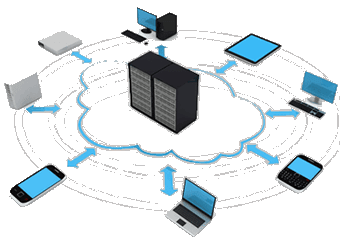
\includegraphics[width=0.60\textwidth]{images/png/VirtualServer.png} % tu archivo WEBP
                    \caption{Representación conceptual de la virtualización en la nube}
                    \label{fig:webp}
                \end{figure}
                \item \textbf{Virtualización de Escritorio}: Permite que los entornos de escritorio se ejecuten en un servidor centralizado y sean accesibles de manera remota desde cualquier dispositivo cliente. Esto proporciona a las organizaciones una forma segura de administrar estaciones de trabajo, facilitar el acceso móvil y reducir los costos de hardware en los puntos finales.
                \begin{figure}[h]
                    \centering
                    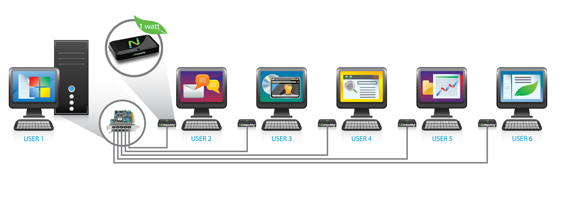
\includegraphics[width=0.7\textwidth]{images/png/VirtualDesk.png} % tu archivo WEBP
                    \caption{Representación conceptual de la virtualización en la nube}
                    \label{fig:webp}
                \end{figure}
                \item \textbf{Virtualización de Redes}: Emula componentes de red como routers, switches y firewalls en entornos virtuales, proporcionando redes lógicas independientes de la infraestructura física. Esto simplifica la gestión de redes complejas, mejora la seguridad mediante la segmentación y facilita la creación de redes aisladas para entornos de prueba y producción.
                \begin{figure}[h]
                    \centering
                    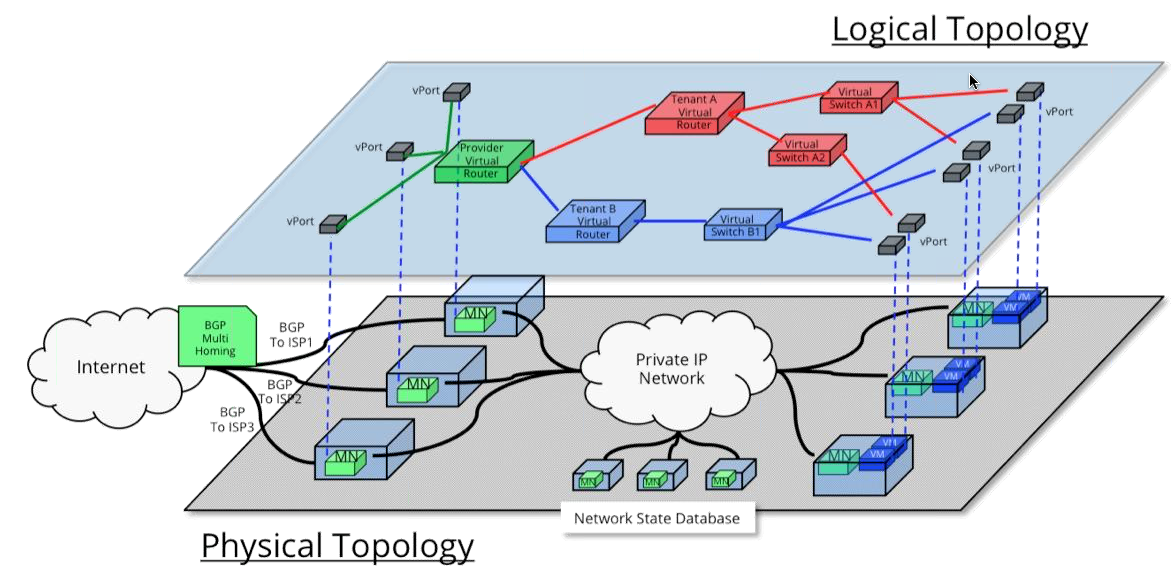
\includegraphics[width=0.75\textwidth]{images/png/VirtualNetwork.png} % tu archivo WEBP
                    \caption{Representación conceptual de la virtualización en la nube}
                    \label{fig:webp}
                \end{figure}
            \end{itemize}
            
        \subsection{Herramientas de Virtualización}
            En el mercado actual existen diversas soluciones de virtualización que proporcionan plataformas robustas y versátiles para la creación y gestión de entornos virtualizados. Entre las herramientas más destacadas se encuentran:
            
            \begin{itemize}
                \item \textbf{VMware vSphere}: Es una de las plataformas de virtualización de servidores más utilizadas en entornos empresariales. Proporciona una infraestructura completa de virtualización que incluye administración centralizada, migración en vivo de máquinas virtuales (\textit{vMotion}) y alta disponibilidad para entornos críticos.
                \item \textbf{Microsoft Hyper-V}: Es la solución de virtualización integrada en los sistemas operativos Windows Server. Permite ejecutar múltiples máquinas virtuales en un único host físico, soportando entornos de nube híbrida y ofreciendo integración nativa con herramientas de administración de Microsoft.
                \item \textbf{KVM (Kernel-based Virtual Machine)}: Es una tecnología de virtualización de código abierto integrada en el núcleo de Linux. Ofrece un alto rendimiento y es compatible con diversas distribuciones Linux, siendo una opción popular en entornos de código abierto y despliegues de nubes privadas.
                \item \textbf{VirtualBox}: Es un software de virtualización gratuito y de código abierto que permite ejecutar múltiples sistemas operativos en un entorno de escritorio. Es ideal para entornos de prueba, desarrollo y formación, al proporcionar una interfaz amigable y soporte para diferentes sistemas operativos invitados.
            \end{itemize}
        
        \subsection{Contenedores y su Aplicación en la Nube}
            Los contenedores representan una evolución significativa en la forma de desplegar y gestionar aplicaciones en entornos de computación en la nube. A diferencia de los métodos tradicionales de virtualización, los contenedores permiten empaquetar aplicaciones junto con sus bibliotecas y dependencias en un entorno aislado, asegurando la consistencia y portabilidad en distintas plataformas y sistemas operativos. Esta característica ha impulsado la adopción de los contenedores como una solución eficiente para implementar arquitecturas de microservicios, donde cada componente de una aplicación puede desplegarse, actualizarse y escalarse de manera independiente, mejorando así, la agilidad en el ciclo de vida del desarrollo de software.

            En el contexto de la computación en la nube, los contenedores ofrecen importantes ventajas en términos de eficiencia de recursos y velocidad de implementación. La ligereza de los contenedores permite iniciar instancias en cuestión de segundos, facilitando el escalado automático de aplicaciones en respuesta a la demanda del usuario. Además, la gestión centralizada de los contenedores mediante plataformas de orquestación, combinada con prácticas de integración y entrega continua (CI/CD), optimiza los procesos de desarrollo y operación, habilitando entornos altamente dinámicos y resilientes en infraestructuras multicloud o híbridas.
            
            \subsubsection{Diferencias entre Contenedores y Máquinas Virtuales}
                A pesar de que tanto los contenedores como las máquinas virtuales (VM) proporcionan mecanismos de aislamiento para ejecutar múltiples aplicaciones en un solo servidor físico, existen diferencias fundamentales en su arquitectura, rendimiento y casos de uso que es importante considerar al diseñar soluciones en la nube.
                    
                Las máquinas virtuales emulan completamente el hardware físico a través de un hipervisor, lo que permite ejecutar varios sistemas operativos invitados, cada uno con su propio kernel y recursos dedicados, como memoria y almacenamiento. Esta arquitectura proporciona un aislamiento robusto y un entorno operativo completamente independiente, lo que es ideal para ejecutar aplicaciones que requieren distintos sistemas operativos o configuraciones específicas de hardware. Sin embargo, este enfoque implica un mayor consumo de recursos, ya que cada VM debe cargar su propio sistema operativo, lo que incrementa el uso de CPU, memoria y espacio en disco, además de tiempos de arranque más prolongados.
                    
                Por el contrario, los contenedores operan a nivel del sistema operativo y comparten el mismo kernel del sistema anfitrión. Esto significa que cada contenedor encapsula únicamente la aplicación y sus dependencias necesarias, lo que reduce significativamente la sobrecarga en comparación con las VM. Los contenedores son ligeros, rápidos de iniciar y escalar, lo que los convierte en una solución ideal para entornos de desarrollo ágiles, despliegue continuo y arquitecturas basadas en microservicios. Sin embargo, el compartir el kernel con el sistema anfitrión puede implicar limitaciones en términos de aislamiento de seguridad y flexibilidad de sistemas operativos distintos dentro de la misma infraestructura.
                    
                Por lo tanto, mientras que las máquinas virtuales ofrecen un entorno más seguro y completamente aislado, adecuado para aplicaciones monolíticas o cargas de trabajo que exigen un control estricto del sistema operativo, los contenedores se orientan a maximizar la eficiencia de los recursos y facilitar el despliegue de aplicaciones distribuidas en la nube, gracias a su arquitectura ligera y modular.
    
                En resumen, las diferencias más importantes entre las máquinas virtuales y los contenedores son:
    
                \begin{itemize}
                    \item Ambos proporcionan aislamiento para ejecutar múltiples aplicaciones en un solo servidor.
                    \item Las máquinas virtuales emulan hardware completo y permiten múltiples sistemas operativos.
                    \item Las VM consumen más recursos y requieren un sistema operativo completo por instancia.
                    \item Los contenedores comparten el \textit{kernel} del sistema anfitrión, siendo más ligeros y rápidos.
                    \item Los contenedores facilitan el despliegue ágil y la escalabilidad en arquitecturas de microservicios.
                    \item Las VM ofrecen mayor aislamiento y son ideales para aplicaciones que exigen entornos específicos.
                    \item Los contenedores tienen menor aislamiento y no permiten diferentes sistemas operativos en la misma infraestructura.
                \end{itemize}
                
            \subsubsection{Orquestación de Contenedores}
                La orquestación de contenedores es un conjunto de procesos y herramientas que permiten la automatización de las operaciones necesarias para gestionar el ciclo de vida de los contenedores en un entorno de producción. Esto incluye tareas como el aprovisionamiento, la implementación, el escalado, la comunicación entre contenedores, la supervisión del estado de las aplicaciones y la recuperación ante fallos. En entornos de nube, donde es común que las aplicaciones se dividan en múltiples microservicios distribuidos en diferentes contenedores, la orquestación se vuelve esencial para garantizar la eficiencia operativa y la disponibilidad continua de los servicios.
                
                Una solución de orquestación proporciona un plano de control que abstrae la complejidad de gestionar múltiples instancias de contenedores que pueden estar distribuidas en distintos nodos físicos o virtuales. Esta abstracción facilita el despliegue de aplicaciones a gran escala, permitiendo que el sistema maneje automáticamente la asignación de recursos, el equilibrio de carga entre contenedores, la actualización de aplicaciones sin tiempo de inactividad y la replicación de servicios para asegurar la alta disponibilidad. Además, las plataformas de orquestación modernas ofrecen capacidades de autoescalado, respondiendo de manera dinámica a los cambios en la carga de trabajo mediante políticas previamente definidas.
                
                Entre los orquestadores de servicios más populares podemos mencionar a:
                \begin{itemize}
                    \item Kubernetes: es ampliamente reconocido por su robustez y flexibilidad, siendo capaz de gestionar entornos altamente complejos y distribuidos. Está diseñado para escalar horizontalmente aplicaciones en miles de contenedores, operando sobre clústeres que pueden extenderse a infraestructuras híbridas o multinube. Su arquitectura modular y su amplia comunidad de soporte lo han convertido en la opción preferida para organizaciones que buscan soluciones de orquestación avanzadas y de gran escala. Kubernetes permite implementar políticas sofisticadas de despliegue, como las actualizaciones progresivas y los retrocesos automáticos, lo que lo hace ideal para escenarios de integración y entrega continua (CI/CD).
                    \item Docker Swarm: Sistema de orquestación integrado en Docker, que ofrece una solución de orquestación más sencilla e integrada directamente en el ecosistema Docker. Su principal ventaja radica en la facilidad de configuración y uso, permitiendo la creación rápida de clústeres de contenedores con un esfuerzo administrativo mínimo. Docker Swarm es adecuado para entornos que requieren una gestión básica de contenedores y que priorizan la simplicidad sobre la personalización avanzada. Si bien no proporciona todas las capacidades sofisticadas de Kubernetes, su curva de aprendizaje es menor, lo que lo convierte en una opción atractiva para pequeñas y medianas implementaciones o para usuarios que recién comienzan a adoptar la contenedorización y la orquestación.
                \end{itemize}

                Por lo tanto, la orquestación de contenedores es fundamental para la gestión eficiente de aplicaciones modernas en la nube, y la elección de la plataforma adecuada dependerá de los requisitos específicos de cada entorno, el nivel de complejidad de las aplicaciones, y la experiencia técnica del equipo de desarrollo y operaciones.
    
        \subsection{Almacenamiento Distribuido en la Nube}
            El almacenamiento distribuido en la nube es una arquitectura clave para la gestión y el acceso a grandes volúmenes de datos en entornos modernos. Este modelo permite almacenar y distribuir datos de manera fragmentada y redundante a través de múltiples servidores o nodos que se encuentran interconectados mediante redes de alta velocidad. Su diseño permite garantizar la alta disponibilidad y la tolerancia a fallos, incluso en situaciones donde uno o varios nodos puedan experimentar interrupciones o caídas de servicio. Al distribuir la información de esta manera, se minimizan los puntos únicos de fallo y se asegura la continuidad del acceso a los datos en todo momento.
            
            Además de la disponibilidad, el almacenamiento distribuido contribuye significativamente a la escalabilidad de las infraestructuras en la nube. A medida que aumenta la demanda de almacenamiento por parte de los usuarios o aplicaciones, se pueden añadir nuevos nodos al sistema sin afectar el funcionamiento general ni requerir una reestructuración compleja. Esta elasticidad permite a las organizaciones escalar de manera horizontal, aumentando la capacidad de almacenamiento y el rendimiento sin interrupciones, y adaptándose a los requisitos cambiantes de los entornos de trabajo dinámicos.
            
            \subsubsection{Beneficios}
                Los sistemas de almacenamiento distribuido ofrecen una serie de ventajas técnicas y operativas que los convierten en la solución preferida en la computación en la nube. Estos beneficios permiten abordar retos tradicionales asociados al almacenamiento centralizado, como la limitación de recursos y la vulnerabilidad frente a fallos únicos.
                
                \begin{itemize}
                    \item \textbf{Acceso Rápido}: La arquitectura distribuida permite que los datos sean accedidos simultáneamente desde varios nodos ubicados en diferentes regiones geográficas, lo que optimiza los tiempos de respuesta y reduce la latencia en la entrega de información. Este acceso paralelo es especialmente útil en aplicaciones que requieren alta disponibilidad de datos en tiempo real, como los servicios de transmisión de contenido multimedia o aplicaciones financieras de alto rendimiento.        
                    \item \textbf{Seguridad}: Los sistemas distribuidos incluyen mecanismos de replicación de datos, en los que la información se almacena de manera redundante en múltiples nodos. Esto asegura la integridad de los datos y protege contra la pérdida de información debido a fallos de hardware o ataques maliciosos. Además, muchas plataformas integran cifrado de datos en tránsito y en reposo, garantizando la confidencialidad y el cumplimiento de regulaciones de seguridad como el RGPD o HIPAA.
                \end{itemize}
                
            \subsubsection{Ejemplos de Almacenamiento Distribuido}
                Las plataformas de almacenamiento distribuido disponibles en el mercado ofrecen soluciones robustas y escalables que han sido adoptadas en diferentes industrias por su fiabilidad y capacidad de integración con servicios en la nube. Estos sistemas suelen emplear tecnologías de replicación y fragmentación avanzada, combinadas con algoritmos de balanceo de carga y consistencia de datos.
                
                \begin{itemize}
                    \item \textbf{Amazon S3}: Amazon Simple Storage Service (S3) es un servicio de almacenamiento de objetos altamente escalable que ofrece disponibilidad del 99.99\% y durabilidad de hasta 11 nueves (99.999999999\%). La arquitectura de S3 permite almacenar objetos en diferentes regiones y zonas de disponibilidad, lo que garantiza la continuidad del servicio y la resistencia a desastres naturales o fallos localizados. Además, ofrece controles granulares de acceso, versiones de objetos y políticas de ciclo de vida para la gestión eficiente del almacenamiento.
                    \item \textbf{Google Cloud Storage}: Es la solución de almacenamiento distribuido de Google, diseñada para almacenar datos de forma redundante en múltiples ubicaciones físicas, asegurando una alta disponibilidad y consistencia. Soporta almacenamiento multirregional y regional, permitiendo a las organizaciones elegir entre priorizar la disponibilidad o la localización geográfica. Asimismo, ofrece integración nativa con los servicios de \textit{Big Data} de Google, como \textit{BigQuery}, facilitando el análisis masivo de datos almacenados sin la necesidad de procesos de migración complejos.        
                    \item \textbf{Apache Hadoop HDFS}: \textit{Hadoop Distributed File System} (HDFS) es un sistema de archivos distribuido utilizado principalmente en el procesamiento y almacenamiento de grandes volúmenes de datos no estructurados. Está diseñado para ejecutarse en hardware estándar, lo que reduce significativamente los costos de implementación en comparación con soluciones propietarias. HDFS divide los datos en bloques que son replicados y distribuidos en diferentes nodos, mejorando la tolerancia a fallos y facilitando el procesamiento paralelo mediante modelos como MapReduce.
                \end{itemize}
                
            \subsubsection{Ejemplos de Almacenamiento Distribuido}
                    \begin{itemize}
                        \item Amazon S3: Servicio de almacenamiento basado en la nube de Amazon Web Services.
                        \item Google Cloud Storage: Plataforma de almacenamiento distribuido de Google.
                        \item Apache Hadoop HDFS: Sistema de archivos distribuido utilizado en análisis de grandes volúmenes de datos.
                    \end{itemize}
                    
        \subsection{Redes Definidas por Software o \textit{Software-Defined Networking} (SDN)}
            Las Redes Definidas por Software, conocidas como SDN por sus siglas en inglés, constituyen un enfoque innovador para la gestión y administración de infraestructuras de red, caracterizado por la separación del plano de control y el plano de datos. Este paradigma ofrece a los administradores un control centralizado de la red a través de un software o controlador, lo que facilita la definición de políticas dinámicas y flexibles para la gestión del tráfico de red. A diferencia de las arquitecturas tradicionales, en las que el hardware de red integra tanto la lógica de control como la de reenvío, en SDN el controlador toma decisiones de encaminamiento y transmite instrucciones a los dispositivos de red subyacentes.
            
            En el contexto de la computación en la nube, las SDN aportan beneficios significativos, ya que permiten adaptar de manera rápida la infraestructura de red a las necesidades cambiantes de las aplicaciones y los usuarios. Esto es fundamental en entornos donde la elasticidad, la automatización y el escalado dinámico son requisitos clave. Las SDN facilitan la creación de redes virtuales personalizadas que pueden ser aprovisionadas bajo demanda, mejorando la eficiencia operativa y reduciendo la dependencia del hardware propietario. Esta capacidad es especialmente relevante en despliegues de nubes públicas, privadas o híbridas, donde la gestión de redes segmentadas y la implementación de políticas de seguridad específicas requieren una administración ágil y centralizada.
            
            \subsubsection{Beneficios}
                El uso de SDN en la nube ofrece diversas ventajas que optimizan la gestión de las redes, mejoran la calidad del servicio y aumentan la seguridad. La flexibilidad de SDN permite una implementación ágil de nuevas políticas de red y una adaptación inmediata a los cambios en la demanda de los recursos.
                
                \begin{itemize}
                    \item \textbf{Mayor Control}: La centralización de la inteligencia de red en un controlador SDN permite definir y aplicar políticas precisas para la gestión del tráfico, el balanceo de carga y la asignación de recursos de red. Esto facilita una administración coherente y simplificada en comparación con los modelos tradicionales, donde cada dispositivo requiere configuración individualizada. Además, el enfoque programable de SDN posibilita la automatización de tareas, como la asignación dinámica de ancho de banda o la priorización de aplicaciones críticas.
                    
                    \item \textbf{Reducción de Costos}: Las SDN minimizan la necesidad de invertir en hardware especializado, permitiendo utilizar dispositivos de red básicos, conocidos como switches de propósito general, mientras que las decisiones de control se trasladan al software. Esto reduce los costos de adquisición y mantenimiento del hardware, y permite un aprovechamiento más eficiente de los recursos de red existentes. Asimismo, la automatización y el aprovisionamiento centralizado disminuyen el tiempo y los costos operativos asociados a la configuración y gestión manual de la red.
                \end{itemize}
            
            \subsubsection{Tecnologías Asociadas a SDN}
                Existen diferentes tecnologías y soluciones que implementan el paradigma SDN, proporcionando funcionalidades avanzadas para el control, la seguridad y la automatización de las redes. Estas tecnologías permiten que la arquitectura SDN sea adoptada en diferentes entornos, desde centros de datos empresariales hasta redes de proveedores de servicios.
            
                \begin{itemize}
                    \item \textbf{OpenFlow}: Es el protocolo estándar más utilizado en las implementaciones de SDN. OpenFlow define cómo se comunican el controlador SDN y los dispositivos de red (switches y routers) para gestionar el flujo de tráfico. Facilita la creación de reglas detalladas que determinan cómo se deben manejar los paquetes, brindando un control granular y dinámico sobre el comportamiento de la red.
                    
                    \item \textbf{Cisco ACI (Application Centric Infrastructure)}: Es una solución de Cisco que proporciona una arquitectura de red SDN centrada en la aplicación. Cisco ACI automatiza la provisión de políticas de red y de seguridad en centros de datos y nubes híbridas, simplificando la administración de la red al abstraer la complejidad de la infraestructura física. Además, integra funcionalidades de análisis de tráfico y monitoreo para mejorar la visibilidad y el rendimiento de la red.
                    
                    \item \textbf{VMware NSX}: Es la plataforma de virtualización de redes de VMware que permite construir redes lógicas independientes de la infraestructura física subyacente. VMware NSX ofrece servicios de red avanzados, como firewalls distribuidos, VPN, balanceo de carga y microsegmentación, facilitando la implementación de políticas de seguridad granular en entornos de nube privada y pública. Su integración con soluciones de virtualización y automatización convierte a NSX en una herramienta clave para arquitecturas de nube definidas por software.
                \end{itemize}

        \subsection{Computación sin Servidor (Serverless Computing)}
            La computación sin servidor, o \textit{Serverless Computing}, representa un modelo de ejecución en la nube donde el aprovisionamiento, la administración y la escalabilidad de la infraestructura subyacente son gestionados completamente por el proveedor del servicio. En este paradigma, los desarrolladores pueden concentrarse exclusivamente en el código y la lógica de negocio de sus aplicaciones, sin preocuparse por los aspectos relacionados con la configuración o el mantenimiento de los servidores físicos o virtuales. La arquitectura serverless responde automáticamente a los eventos, ejecutando funciones en tiempo real bajo demanda, lo que permite una asignación dinámica y precisa de los recursos según la necesidad del sistema o el usuario final.
            
            Uno de los principales diferenciadores de este modelo es su capacidad para optimizar el costo operativo, ya que se basa en un esquema de facturación bajo demanda, donde los usuarios solo pagan por el tiempo de ejecución y el número de invocaciones de las funciones. Esto contrasta con los enfoques tradicionales de infraestructura en la nube, en los que los recursos deben ser aprovisionados y mantenidos de forma continua, incluso si no se están utilizando activamente. Además, el modelo serverless se integra de manera natural con arquitecturas basadas en microservicios y flujos de eventos, facilitando el desarrollo de sistemas altamente escalables, resilientes y orientados a eventos.
            
            \subsubsection{Plataformas de Serverless Computing}
                El ecosistema de la computación sin servidor incluye diversas plataformas ofrecidas por proveedores de servicios en la nube, las cuales proporcionan entornos flexibles para el desarrollo y la ejecución de funciones. Estas plataformas abstraen por completo la complejidad de la infraestructura, permitiendo al usuario centrarse en la lógica de sus aplicaciones.
                
                \begin{itemize}
                    \item \textbf{AWS Lambda}: Es una de las soluciones serverless más maduras del mercado, desarrollada por Amazon Web Services. Permite ejecutar funciones en respuesta a eventos como modificaciones en datos almacenados en Amazon S3, actualizaciones en bases de datos DynamoDB o eventos provenientes de flujos de datos en tiempo real. Lambda soporta múltiples lenguajes de programación, incluyendo Python, Node.js, Java y Go, y ofrece integración nativa con el resto de los servicios de AWS. Además, proporciona escalabilidad automática, ejecutando múltiples instancias de funciones en paralelo cuando es necesario, y gestionando la tolerancia a fallos de forma transparente para el usuario.                   
                    \item \textbf{Google Cloud Functions}: Esta plataforma de Google permite el despliegue de funciones en la nube como respuesta a eventos provenientes de servicios como Google Cloud Storage, Firestore o Pub/Sub. Se integra de manera sencilla con otros productos del ecosistema de Google Cloud, así como con herramientas de desarrollo modernas como Firebase. Cloud Functions ofrece un modelo de escalado basado en la carga de trabajo entrante y soporta diversos lenguajes, incluyendo JavaScript (Node.js), Python y Go. Asimismo, proporciona características avanzadas de control de acceso, registro de auditorías y supervisión de métricas para garantizar el cumplimiento de políticas de seguridad y conformidad.
                \end{itemize}
                        
        \subsection{Técnicas de Automatización}
            Las técnicas de automatización en la computación en la nube permiten gestionar de forma eficiente y controlada los recursos y procesos dentro de una infraestructura tecnológica. Estas técnicas contribuyen a reducir el esfuerzo manual en la administración de sistemas, incrementando la velocidad de despliegue de servicios, mejorando la consistencia de las configuraciones y disminuyendo la posibilidad de errores humanos. La automatización es un componente fundamental en la implementación de prácticas DevOps, facilitando la entrega continua (\textit{Continuous Delivery}) y la integración continua (\textit{Continuous Integration}), además de potenciar la infraestructura como código (\textit{Infrastructure as Code, IaC}).
            
            En los entornos de nube modernos, la automatización se aplica en diversas áreas, como la configuración y gestión de servidores, el aprovisionamiento de recursos virtuales, la seguridad de los datos y la administración de redes. Las herramientas y técnicas de automatización permiten a las organizaciones definir reglas y políticas que se ejecutan de manera automática para mantener la infraestructura alineada con los requisitos operativos y de seguridad. Además, la automatización es clave para lograr la elasticidad en la nube, ajustando los recursos de forma dinámica según la demanda del sistema o del usuario final.
            
            \begin{itemize}
                \item \textbf{Cifrado de Datos}: El cifrado es una técnica esencial para proteger la confidencialidad de los datos almacenados y en tránsito dentro de las infraestructuras de nube. Mediante algoritmos criptográficos avanzados como AES (Advanced Encryption Standard) o RSA (Rivest-Shamir-Adleman), los datos se transforman en un formato ilegible para usuarios no autorizados. La automatización del cifrado permite que los datos sean encriptados de manera transparente durante su transferencia entre servicios o cuando son almacenados en repositorios distribuidos, asegurando el cumplimiento de normativas internacionales como el Reglamento General de Protección de Datos (RGPD) y la Ley de Portabilidad y Responsabilidad del Seguro de Salud (HIPAA).            
                \item \textbf{Gestión de Identidad y Accesos (IAM)}: La gestión automatizada de identidades y accesos permite controlar quién puede acceder a los recursos en la nube y bajo qué condiciones. Las soluciones IAM automatizan la asignación de roles y políticas de acceso basadas en principios de mínimo privilegio y segregación de funciones, reduciendo la exposición a riesgos de seguridad. Estas políticas se integran con directorios de autenticación como Azure Active Directory o AWS IAM y permiten aplicar autenticación multifactor (MFA), gestión de sesiones y auditorías de acceso de manera automática y centralizada.            
                \item \textbf{Terraform}: Terraform es una herramienta de infraestructura como código (IaC) que permite definir y aprovisionar recursos de infraestructura a través de archivos de configuración en formato declarativo. Soporta múltiples proveedores de servicios en la nube, como AWS, Azure y Google Cloud Platform, lo que facilita la creación de infraestructuras híbridas o multicloud. Terraform automatiza la gestión del ciclo de vida de los recursos, permitiendo la creación, actualización y eliminación de componentes de infraestructura mediante la ejecución de planes controlados y auditable.            
                \item \textbf{Ansible}: Ansible es una plataforma de automatización de código abierto que permite gestionar la configuración de servidores, la implementación de aplicaciones y la orquestación de tareas administrativas. Utiliza un lenguaje de configuración sencillo basado en YAML, lo que facilita la definición de \textit{playbooks} para ejecutar procesos repetitivos sin intervención manual. Ansible no requiere la instalación de agentes en los nodos administrados y se integra fácilmente con sistemas de control de versiones y flujos de CI/CD, garantizando despliegues coherentes y reproducibles.
                \item \textbf{Cloudflare}: Cloudflare proporciona soluciones automatizadas para mejorar la seguridad, el rendimiento y la disponibilidad de aplicaciones web y servicios en línea. Su plataforma de seguridad protege automáticamente contra ataques DDoS, inyecciones de código y amenazas de bots maliciosos. Además, Cloudflare ofrece una red de entrega de contenido (CDN) que optimiza la distribución de recursos estáticos, acelerando el tiempo de respuesta para usuarios en diferentes ubicaciones geográficas. Las reglas y configuraciones de seguridad en Cloudflare pueden ser automatizadas y gestionadas mediante su API y paneles de control integrados.            
                \item \textbf{IBM Cloud Security}: IBM Cloud Security proporciona un conjunto de herramientas de automatización orientadas a la protección de datos, la gestión de amenazas y la gobernanza de la seguridad en la nube. Ofrece capacidades como la detección automatizada de vulnerabilidades, la aplicación de políticas de cumplimiento regulatorio y el cifrado de datos en entornos de nube pública, privada e híbrida. La plataforma se integra con soluciones de inteligencia de amenazas y análisis de comportamiento, permitiendo una respuesta proactiva y automatizada ante incidentes de seguridad.
            \end{itemize}
            
    \section{Contenedores y su orquestación}
        Los contenedores son unidades estándar de software que empaquetan el código y todas sus dependencias para que la aplicación se ejecute de manera rápida y confiable en diferentes entornos informáticos. Son más ligeros que las máquinas virtuales, ya que no necesitan un sistema operativo adicional. La portabilidad y la eficiencia de los contenedores los han convertido en un componente esencial para las arquitecturas modernas basadas en microservicios.
        
        Los contenedores se utilizan para desarrollar, entregar y operar aplicaciones de manera eficiente, especialmente en entornos de nube, donde la escalabilidad y la eficiencia son importantes. Además, su integración con herramientas de integración continua/despliegue continuo (CI/CD) permite acelerar los ciclos de desarrollo y asegurar consistencia entre entornos de desarrollo, pruebas y producción.
        
        \subsection{Docker - Plataforma de Contenedores}
            Docker es una plataforma de contenedores que permite desarrollar, desplegar y ejecutar aplicaciones en contenedores. Utiliza la virtualización a nivel de sistema operativo para entregar software en paquetes llamados contenedores. Esto simplifica el proceso de despliegue al encapsular la aplicación y sus dependencias en una unidad ejecutable portátil. Docker ofrece herramientas que permiten a los desarrolladores construir imágenes, gestionar registros y ejecutar aplicaciones distribuidas en diferentes entornos.
        
            \subsubsection{Características de Docker}
                Docker ofrece un conjunto de características que han revolucionado el desarrollo y despliegue de aplicaciones, facilitando la creación de entornos consistentes y portables. Estas funcionalidades permiten simplificar la gestión de la infraestructura subyacente, reduciendo la complejidad operativa y acelerando el ciclo de vida del software.

                \begin{itemize}
                    \item \textbf{Portabilidad}: Las aplicaciones en contenedores Docker pueden ejecutarse consistentemente en cualquier entorno, desde equipos de desarrollo locales hasta servidores en la nube. Esto se logra mediante el uso de imágenes inmutables que garantizan que el entorno de ejecución siempre sea el mismo.
                    
                    \item \textbf{Aislamiento}: Cada contenedor se ejecuta de forma independiente, garantizando que los procesos no interfieran entre sí. Esto se implementa mediante namespaces y cgroups del kernel de Linux, ofreciendo un alto grado de seguridad y control sobre los recursos.
                \end{itemize}
            
            \subsubsection{Ventajas de Usar Contenedores}
                El uso de contenedores aporta múltiples beneficios al desarrollo y operación de aplicaciones, optimizando el uso de los recursos del sistema y mejorando la agilidad en la entrega de software. A continuación, se describen las ventajas clave de implementar esta tecnología en entornos de producción.

                \begin{itemize}
                    \item \textbf{Eficiencia de Recursos}: Los contenedores requieren menos recursos que las máquinas virtuales tradicionales porque comparten el núcleo del sistema operativo host y no necesitan su propio sistema operativo completo. Esto reduce el consumo de memoria y CPU, lo que permite ejecutar más instancias en la misma infraestructura física.
                    
                    \item \textbf{Rapidez de Despliegue}: Los contenedores pueden iniciarse en segundos, lo que permite despliegues y escalados rápidos. Esto es especialmente útil en entornos de alta disponibilidad donde se requiere una respuesta inmediata ante picos de demanda.
                \end{itemize}
            
            \subsubsection{Ciclo de Vida del Contenedor en Docker}
                El ciclo de vida de un contenedor en Docker abarca desde la construcción de la imagen hasta su ejecución, monitoreo y eliminación. A continuación, se detallan las principales fases que permiten una gestión efectiva de los contenedores dentro de un entorno controlado.

                \begin{itemize}
                    \item \textbf{Creación de Contenedores}: Desde el desarrollo hasta la producción, Docker proporciona un entorno consistente para que las aplicaciones se ejecuten, facilitando pruebas y reduciendo inconsistencias entre entornos. Para crear una imagen Docker se utiliza un archivo \texttt{Dockerfile}, que contiene instrucciones para construir la imagen.
                
                    \begin{verbatim}
    # Ejemplo básico de Dockerfile
    FROM python:3.9-slim
    WORKDIR /app
    COPY requirements.txt .
    RUN pip install -r requirements.txt
    COPY . .
    CMD ["python", "app.py"]
                    \end{verbatim}
                    
                    Luego, la imagen se construye y se ejecuta con los siguientes comandos:
                    
                    \begin{verbatim}
    docker build -t mi-aplicacion:1.0 .
    docker run -d -p 5000:5000 mi-aplicacion:1.0
                    \end{verbatim}
                
                    \item \textbf{Gestión de Contenedores}: Docker simplifica la gestión de contenedores mediante comandos sencillos y archivos de configuración. Se pueden listar contenedores activos con:
                
                    \begin{verbatim}
    docker ps
                    \end{verbatim}
                
                    Para detener y eliminar contenedores:
                
                    \begin{verbatim}
    docker stop ID_CONTENEDOR
    docker rm ID_CONTENEDOR
                    \end{verbatim}
                
                    Además, las imágenes creadas pueden almacenarse en registros como Docker Hub o Azure Container Registry:
                
                    \begin{verbatim}
    docker tag mi-aplicacion:1.0 usuario/mi-aplicacion:1.0
    docker push usuario/mi-aplicacion:1.0
                    \end{verbatim}
                \end{itemize}
            
            \subsubsection{Seguridad en Contenedores}
                La seguridad en la ejecución de contenedores es fundamental para proteger tanto la integridad de los datos como la estabilidad del entorno de ejecución. Las siguientes prácticas y mecanismos de seguridad ayudan a mitigar riesgos asociados al uso de contenedores en infraestructuras de producción.

                \begin{itemize}
                    \item \textbf{Aislamiento de Contenedores}: Aunque los contenedores comparten el núcleo del sistema operativo, están aislados entre sí, lo que proporciona un nivel de seguridad. Docker recomienda el uso de imágenes oficiales o verificadas y la ejecución de contenedores en usuarios sin privilegios.
                
                    Se puede ejecutar un contenedor sin acceso privilegiado utilizando:
                
                    \begin{verbatim}
    docker run --user 1000:1000 -d mi-aplicacion:1.0
                    \end{verbatim}
                
                    Además, se pueden escanear imágenes en busca de vulnerabilidades con herramientas como \texttt{docker scan}:
                
                    \begin{verbatim}
    docker scan mi-aplicacion:1.0
                    \end{verbatim}
                \end{itemize}
            
        \subsection{Kubernetes - Orquestación de Contenedores}
            Kubernetes es un sistema de orquestación de contenedores de código abierto que automatiza la implementación, el escalado y la gestión de aplicaciones en contenedores. Fue originalmente desarrollado por Google y ahora es mantenido por la Cloud Native Computing Foundation. Su arquitectura modular permite gestionar clústeres de contenedores en entornos de producción de manera eficiente y resiliente.
            
            \subsubsection{Funciones de Kubernetes}
                Kubernetes ofrece una serie de funciones que automatizan la gestión de contenedores a gran escala. Estas capacidades facilitan el despliegue continuo, el balanceo de carga y la resiliencia de las aplicaciones en un clúster distribuido.

                \begin{itemize}
                    \item \textbf{Automatización del Despliegue}: Kubernetes gestiona automáticamente el despliegue y la actualización de contenedores mediante recursos como Deployments y ReplicaSets. Un ejemplo de Deployment en YAML sería:
                
                    \begin{verbatim}
    apiVersion: apps/v1
    kind: Deployment
    metadata:
        name: mi-aplicacion
    spec:
        replicas: 3
        selector:
            matchLabels:
                app: mi-aplicacion
        template:
            metadata:
                labels:
                    app: mi-aplicacion
            spec:
                containers:
                - name: mi-aplicacion
                  image: usuario/mi-aplicacion:1.0
                  ports:
                  - containerPort: 5000
                    \end{verbatim}
                
                    \item \textbf{Balanceo de Carga}: Distribuye automáticamente el tráfico de red entre los contenedores de una aplicación utilizando objetos de tipo \texttt{Service}. Ejemplo de un Service tipo ClusterIP:
                
                    \begin{verbatim}
    apiVersion: v1
    kind: Service
    metadata:
        name: mi-aplicacion-service
    spec:
        selector:
            app: mi-aplicacion
        ports:
            - protocol: TCP
              port: 80
              targetPort: 5000
                    \end{verbatim}
                \end{itemize}
            
            \subsubsection{Arquitectura de Kubernetes}
                La arquitectura de Kubernetes se compone de diferentes elementos que interactúan para proporcionar un entorno flexible y escalable para la ejecución de contenedores. A continuación, se describen sus principales componentes y su función dentro del clúster.

                \begin{itemize}
                    \item \textbf{Pods}: La unidad más pequeña en Kubernetes, que puede contener uno o más contenedores que comparten almacenamiento y red. Se crean automáticamente mediante los Deployments.
                
                    \item \textbf{Nodes}: Son servidores físicos o virtuales que alojan los Pods y proporcionan los recursos de cómputo necesarios para ejecutar las aplicaciones.
                
                    \item \textbf{Master (Control Plane)}: Es el conjunto de componentes que gestiona el estado del clúster, programando Pods y supervisando el estado general del sistema. Incluye el API Server, Controller Manager, Scheduler y etcd.
                \end{itemize}
            
            \subsubsection{Beneficios de Kubernetes en Ambientes de Producción}
                Kubernetes se ha convertido en el estándar de facto para la orquestación de contenedores debido a sus ventajas operativas y de escalabilidad. A continuación, se detallan los principales beneficios que ofrece en entornos de producción.

                \begin{itemize}
                    \item \textbf{Escalabilidad Automática}: Kubernetes puede escalar aplicaciones automáticamente mediante el Horizontal Pod Autoscaler (HPA). Ejemplo para escalar un Deployment automáticamente:
                
                    \begin{verbatim}
                    kubectl autoscale deployment mi-aplicacion --cpu-percent=50 --min=1 --max=10
                    \end{verbatim}
                
                    \item \textbf{Recuperación Automática}: Kubernetes reinicia contenedores que fallan, reemplaza Pods defectuosos y reprograma Pods en Nodes disponibles en caso de caídas. Los Liveness y Readiness Probes permiten verificar el estado de los contenedores:
                
                    \begin{verbatim}
    livenessProbe:
        httpGet:
            path: /healthz
            port: 5000
        initialDelaySeconds: 3
        periodSeconds: 10
                    \end{verbatim}
                \end{itemize}
            
            \subsection{Docker Compose y Kubernetes YAML}
                La gestión de contenedores en entornos de producción requiere herramientas que faciliten la definición, el despliegue y la orquestación de múltiples servicios. Tanto Docker Compose como Kubernetes utilizan archivos en formato YAML para declarar la configuración de las aplicaciones, describiendo aspectos clave como los servicios que la componen, sus dependencias, las redes, volúmenes, políticas de escalado y otras directrices operativas.

                Docker Compose se orienta principalmente a simplificar la definición y ejecución de aplicaciones multi-contenedor en entornos de desarrollo o pruebas, aunque también puede utilizarse en escenarios de producción pequeños o medianos. Por otro lado, Kubernetes se ha convertido en el estándar de facto para la orquestación de contenedores a gran escala, ofreciendo un control más granular sobre el ciclo de vida de las aplicaciones, el escalado automático, la distribución de la carga y la recuperación ante fallos.

            \subsubsection{Docker Compose}
                Docker Compose simplifica la ejecución de aplicaciones que requieren múltiples contenedores, proporcionando una sintaxis declarativa y sencilla para definir y administrar los distintos servicios que componen una aplicación. Utiliza un archivo YAML para configurar los servicios de la aplicación, especificando redes, volúmenes y dependencias. Ejemplo de un archivo \texttt{docker-compose.yml} básico:
            
                \begin{verbatim}
    version: '3'
    services:
        web:
            image: mi-aplicacion:1.0
            ports:
                - "5000:5000"
            depends_on:
                - db
        db:
            image: postgres:13
            environment:
                POSTGRES_USER: usuario
                POSTGRES_PASSWORD: password
                \end{verbatim}
                
                Se puede desplegar la pila con el siguiente comando:
                
                \begin{verbatim}
    docker-compose up -d
                \end{verbatim}
            
            \subsubsection{Kubernetes YAML}
                Kubernetes permite definir sus recursos de manera declarativa a través de archivos YAML, facilitando la automatización y el control de la infraestructura mediante la gestión de versiones, además de su mantenimiento y la reproducibilidad de los despliegues.
                
                Los recursos típicos incluyen Pods, Deployments, Services y ConfigMaps. Se aplican al clúster con el siguiente comando:
            
                \begin{verbatim}
    kubectl apply -f deployment.yaml
                \end{verbatim}
            
            \subsection{Seguridades en Kubernetes}
                Garantizar la seguridad en un clúster de Kubernetes implica la aplicación de políticas de acceso, la segmentación de redes y el monitoreo constante de la actividad. Las siguientes medidas contribuyen a fortalecer la postura de seguridad en estos entornos.

                \begin{itemize}
                    \item \textbf{Prácticas de Seguridad}: Implementar políticas de seguridad es esencial en Kubernetes. Algunas recomendaciones incluyen el uso de Roles y RoleBindings (RBAC) para controlar el acceso:
                
                    \begin{verbatim}
    kubectl create role developer --verb=get,list,watch --resource=pods
    kubectl create rolebinding developer-binding --role=developer --user=usuario
                    \end{verbatim}
                
                    Además, se recomienda activar Network Policies para limitar la comunicación entre Pods:
                
                    \begin{verbatim}
    apiVersion: networking.k8s.io/v1
    kind: NetworkPolicy
    metadata:
        name: deny-all
    spec:
        podSelector: {}
        policyTypes:
        - Ingress
                    \end{verbatim}
                \end{itemize}
                
            \subsection{Networking en Docker y Kubernetes}
            
            \subsubsection{Redes en Docker}
                Docker proporciona un sistema de redes virtuales que facilita la comunicación entre contenedores, tanto dentro de un mismo host como a través de múltiples nodos en un entorno distribuido. Estas redes permiten definir reglas de conectividad seguras y eficientes.
                
                Por lo tanto,  Docker permite configurar redes internas para conectar contenedores en el mismo host y entre diferentes hosts. Se pueden crear redes de tipo bridge, overlay o host. Ejemplo de creación de una red bridge:
            
                \begin{verbatim}
    docker network create --driver bridge red-interna
    docker run -d --network red-interna --name app1 mi-aplicacion:1.0
    docker run -d --network red-interna --name app2 mi-aplicacion:1.0
                \end{verbatim}
            
            \subsubsection{Redes en Kubernetes}
                Kubernetes implementa un modelo de red plano, donde todos los Pods dentro del clúster pueden comunicarse entre sí  sin NAT. La configuración de redes y políticas asegura la conectividad controlada y el cumplimiento de requisitos de seguridad y rendimiento.
                
                Se recomienda el uso de soluciones CNI (Container Network Interface) como Calico o Flannel para la gestión de redes. Para crear una red de servicios entre Pods, se usa el tipo ClusterIP en los servicios de Kubernetes, como se mostró anteriormente. Además, Ingress Controllers permiten el acceso HTTP/S desde el exterior:
            
                \begin{verbatim}
    apiVersion: networking.k8s.io/v1
    kind: Ingress
    metadata:
        name: mi-aplicacion-ingress
    spec:
        rules:
        - host: mi-aplicacion.dominio.com
            http:
                paths:
                - path: /
                    pathType: Prefix
                    backend:
                        service:
                            name: mi-aplicacion-service
                            port:
                                number: 80
                \end{verbatim}
    \section{SDN}            
        Las SDN representan un avance disruptivo en diseño y administración de infraestructura de red. Este paradigma introduce una revolucionaria arquitectura que desvincula explícitamente el plano del control del plano de datos, permitiendo centralizar la toma de decisiones en cuanto al comportamiento de la red, mientras que dispositivos de red bajo (switches, routers, firewalls, entre otros) se reducen a cumplir órdenes dadas por un controlador centralizado.

        En los modelos tradicionales, cada dispositivo de red opera de forma autónoma, integrando simultáneamente las funciones de control (planificación y decisión sobre el encaminamiento del tráfico) y de reenvío de paquetes (procesamiento y envío de los datos). Esta arquitectura distribuida incrementa la complejidad de la gestión, dificulta la aplicación coherente de políticas de red y limita la capacidad de escalar de manera eficiente en entornos dinámicos como los centros de datos modernos y las nubes públicas o privadas.
        
        SDN resuelve estas limitaciones mediante la abstracción del plano de control, consolidando la inteligencia de la red en un software denominado \textit{controlador SDN}, el cual actúa como cerebro del sistema. Este controlador gestiona globalmente el comportamiento de la red, define las reglas de enrutamiento y configuración, y establece políticas de calidad de servicio (\textit{QoS}), seguridad y segmentación. Los dispositivos de red, a su vez, funcionan como simples \textit{forwarders} o planos de datos, obedeciendo las instrucciones que reciben a través de protocolos estándar como OpenFlow o interfaces de programación de aplicaciones (APIs).
        
        Una de las principales fortalezas de SDN es su programabilidad. Con interfaces abiertas y estandarizadas, como las RESTful APIs, SDN permite a los desarrolladores crear aplicaciones de red que automatizan tareas, aplican control de tráfico inteligente y orquestan dinámicamente los recursos de red. Esta capacidad programable convierte la red en un recurso ágil y flexible, alineado con los principios de la computación en la nube y la virtualización de funciones de red (NFV).
        
        Además, SDN facilita el manejo heterogéneo y multi-proveedor de infraestructura de red desde un único punto de control, evitando la dependencia en soluciones propietarias (\textit{vendor lock-in}) y fomentando la interoperabilidad. De esta manera, se simplifica la implementación de políticas globales de seguridad, el monitoreo en tiempo real de los flujos de datos y la aplicación de medidas de cumplimiento normativo (\textit{compliance}) de manera más sencilla y eficiente.
        
        En el contexto de los centros de datos definidos por software (SDDC), SDN desempeña un papel fundamental al facilitar redes virtualizadas que soportan cargas de trabajo distribuidas, proporcionando conectividad escalable y segura para aplicaciones modernas como servicios de microservicios, IoT, Big Data y 5G.
        
        \subsection{Objetivos de SDN}
            La emergencia del Software-Defined Networking (\textit{Software-Defined Networking, SDN}) se debe a la demanda para superar la restricción en la arquitectura tradicional de red, que es dispositivo propósito específico basada y que combina en forma rígida el plano de datos y el plano del control. Esta rígida restricción ha obstaculizado en el pasado la capacidad para que las organizaciones escalen, automaten y mejoren sus redes en forma flexible y dinámica. Por este motivo, SDN propone un cambio revolucionario en la forma en que se diseñan y se manejan las redes, alineándose a la nueva demanda impuesta por la virtualización, la computación en la nube y el crecimiento explosivo de las aplicaciones distribuidas.

            Los objetivos primarios del SDN trascienden el manejo básico del tráfico, proponiendo un modelo más flexible, programable y adaptable que pueda responder activamente a los avances tecnológicos y a los demandas de negocios emergentes. Los siguientes son los propósitos más relevantes del SDN en este sentido:

        \begin{itemize}        
            \item \textbf{Abstracción y Centralización del Control de Red:} SDN busca abstraer la lógica de control de la red del hardware subyacente, proporcionando una vista lógica centralizada que facilite la toma de decisiones a nivel global. Esta abstracción permite a los administradores definir políticas de tráfico, seguridad y calidad de servicio (QoS) desde un único punto de control, sin depender de la configuración manual y aislada de cada dispositivo de red físico.
            \item \textbf{Acelerar la Innovación en la Infraestructura de Red:} La arquitectura SDN está diseñada para ser abierta y extensible, lo que promueve la innovación tanto en el desarrollo de nuevos protocolos de red como en la integración con aplicaciones empresariales y de nube. Mediante APIs estandarizadas (como RESTful APIs) y controladores programables, SDN permite experimentar con algoritmos de enrutamiento dinámico, balanceo de carga inteligente y políticas de seguridad adaptativas, sin necesidad de reemplazar el hardware.
            \item \textbf{Facilitar la Automatización y Orquestación de Servicios de Red:} SDN tiene como objetivo eliminar la intervención manual en la provisión y gestión de los recursos de red. A través de la automatización, se reduce la complejidad operativa y se incrementa la consistencia en la aplicación de políticas. La orquestación de servicios de red posibilita la creación y despliegue automático de redes virtuales, integradas con procesos de DevOps, CI/CD y administración de entornos multicloud.
            \item \textbf{Mejorar la Escalabilidad y la Elasticidad de la Red:} En los entornos actuales de centros de datos y redes de proveedores de servicios, la capacidad de escalar recursos de red de forma elástica es esencial para responder a variaciones dinámicas en la carga de trabajo. SDN permite gestionar y escalar redes de manera eficiente, ajustando dinámicamente los recursos asignados a flujos de datos, aplicaciones o usuarios, sin afectar el rendimiento general ni requerir reconfiguraciones manuales.
            \item \textbf{Incrementar la Visibilidad y el Monitoreo del Tráfico de Red:} SDN proporciona herramientas avanzadas de monitoreo y análisis del tráfico, lo que facilita la detección de cuellos de botella, la identificación de patrones anómalos y la implementación de mecanismos de respuesta ante incidentes de seguridad. La visibilidad granular y en tiempo real mejora la capacidad de tomar decisiones informadas y garantiza la calidad de servicio requerida por las aplicaciones críticas.
            \item \textbf{Asegurar la Interoperabilidad y la Independencia de Proveedores:} Al estandarizar la comunicación entre el plano de control y el plano de datos (por ejemplo, mediante protocolos como OpenFlow), SDN permite evitar el lock-in tecnológico y fomenta la interoperabilidad entre dispositivos de diferentes fabricantes. Esta apertura ofrece a las organizaciones la flexibilidad de seleccionar soluciones de red basadas en sus necesidades y presupuestos específicos.
        \end{itemize}
                
        \subsection{Componentes Clave de SDN}
            Las Redes Definidas por Software (SDN) están compuestas por varios elementos fundamentales que trabajan en conjunto para ofrecer un entorno de red centralizado, programable y flexible. Comprender estos componentes es esencial para entender cómo funciona el ecosistema SDN y cómo se integra en la infraestructura tecnológica actual. A continuación, se describen los principales componentes que conforman una arquitectura SDN típica:

            \begin{itemize}
                \item \textbf{Controlador SDN}: Considerado el cerebro de una red SDN, el controlador centraliza la inteligencia y toma decisiones sobre el comportamiento de la red. Proporciona la interfaz entre las aplicaciones y los dispositivos de red subyacentes, gestionando el flujo de tráfico y garantizando una operación coherente y optimizada.
                \item \textbf{Dispositivos de Red SDN}: Estos incluyen switches y routers diseñados para ser controlados de manera centralizada por el controlador SDN. A diferencia de los dispositivos tradicionales, su funcionalidad se limita principalmente al reenvío de paquetes, mientras que las decisiones de enrutamiento y políticas de red se definen desde el controlador.
            \end{itemize}
        
        \subsection{Ventajas de Implementar SDN}
            La implementación de SDN ofrece una amplia gama de beneficios para las organizaciones que buscan modernizar su infraestructura de red y responder a las demandas del entorno digital actual. Gracias a su arquitectura centralizada y programable, SDN permite a los administradores gestionar sus redes de manera más eficiente, flexible y segura. A continuación, se detallan algunas de las principales ventajas que ofrece esta tecnología:

            \begin{itemize}
                \item \textbf{Agilidad y Flexibilidad}: SDN proporciona a los administradores de red la capacidad de adaptar rápidamente la infraestructura de red en función de las necesidades cambiantes del negocio. Esto incluye la implementación de nuevas aplicaciones, la gestión de incrementos en el tráfico de datos o la respuesta a eventos imprevistos sin necesidad de realizar cambios físicos en el hardware.
                \item \textbf{Optimización de Recursos}: Al centralizar y automatizar la gestión de la red, SDN permite un uso más eficiente de los recursos disponibles. Esto puede traducirse en una reducción significativa de los costos operativos (OPEX) y de capital (CAPEX), al tiempo que se mejora el rendimiento y la disponibilidad de los servicios de red.
            \end{itemize}
        
        \subsection{SDN en Centros de Datos}
            Los centros de datos modernos son entornos dinámicos y altamente exigentes que requieren soluciones de red avanzadas para garantizar la conectividad, seguridad y rendimiento de los servicios alojados. En este contexto, SDN juega un papel crucial al aportar herramientas y capacidades que permiten una gestión más eficiente y flexible de la red. A continuación, se presentan algunas de las aplicaciones más destacadas de SDN en el ámbito de los centros de datos:

            \begin{itemize}
                \item \textbf{Automatización del Centro de Datos}: SDN facilita la automatización de tareas rutinarias dentro del centro de datos, tales como la configuración de la red, la implementación de políticas de seguridad y el balanceo de carga entre servidores. Esta automatización contribuye a reducir errores humanos, mejorar la eficiencia operativa y acelerar la provisión de servicios.
                \item \textbf{Virtualización de Red}: Una de las capacidades más valiosas de SDN es la posibilidad de crear redes virtuales que se superponen a la infraestructura física existente. Esto permite segmentar y proteger diferentes recursos y servicios críticos del negocio sin necesidad de adquirir hardware adicional, favoreciendo así la seguridad y la escalabilidad del entorno de TI.
            \end{itemize}

        \subsubsection{Tecnologías Asociadas a SDN}
            La adopción de SDN ha dado lugar a una serie de tecnologías y soluciones que facilitan su implementación y amplían sus capacidades. Estas tecnologías proporcionan los protocolos, plataformas y herramientas necesarias para gestionar redes de manera centralizada, automatizada y segura, adaptándose a las necesidades específicas de cada organización. A continuación, se describen algunas de las tecnologías más representativas asociadas al ecosistema SDN:
            
            \paragraph{OpenFlow} Es uno de los protocolos estándar más importantes y ampliamente adoptados para la implementación de SDN. OpenFlow define la comunicación entre el plano de control (controlador SDN) y el plano de datos (dispositivos de red), permitiendo al controlador dictar cómo se deben manejar los paquetes de datos en los switches y routers. Gracias a su diseño abierto y estandarizado, OpenFlow ha sido fundamental para promover la interoperabilidad entre diferentes fabricantes y fomentar el desarrollo de soluciones SDN flexibles y escalables.
            
            \paragraph{Cisco ACI} (Application Centric Infrastructure) es la plataforma de automatización de redes desarrollada por Cisco. ACI ofrece un enfoque integral para la gestión de redes, centrado en las aplicaciones, lo que permite a las organizaciones definir políticas de red basadas en los requisitos específicos de cada aplicación. Cisco ACI combina hardware especializado con un plano de control centralizado, brindando visibilidad completa, automatización avanzada y un modelo operativo coherente para redes físicas y virtuales.
            
            \paragraph{VMware NSX} Es la solución de virtualización de redes de VMware, diseñada para proporcionar redes definidas por software en entornos empresariales. NSX permite abstraer la red de la infraestructura física subyacente, ofreciendo una plataforma para crear redes virtuales completas con funciones avanzadas de seguridad, segmentación y automatización. VMware NSX se integra estrechamente con entornos de virtualización de servidores, facilitando la implementación de centros de datos definidos por software (SDDC) y promoviendo una mayor agilidad y eficiencia operativa.
        
        \subsection{Protocolos Utilizados en SDN}
            En el ecosistema de las Redes Definidas por Software (SDN), los protocolos desempeñan un papel fundamental para garantizar una comunicación eficiente y coherente entre los distintos componentes de la red. Estos protocolos son el puente que permite al controlador centralizado comunicarse con los dispositivos de red, como switches y routers, definiendo de manera precisa cómo deben gestionar y dirigir el tráfico de datos.
            
            El desarrollo de protocolos específicos para SDN ha revolucionado la forma en que se administra y opera una red, ya que proporcionan la flexibilidad y dinamismo que las arquitecturas tradicionales no podían ofrecer. Esta evolución ha permitido que los administradores puedan definir políticas y reglas de red desde un punto centralizado, haciendo que la implementación de nuevas aplicaciones o servicios sea mucho más ágil.
            
            Entre los protocolos más utilizados en el ámbito de SDN, OpenFlow destaca como el primero y más adoptado estándar, permitiendo un control granular y dinámico del tráfico de red. Sin embargo, existen otros protocolos que también complementan y amplían las capacidades de las soluciones SDN, facilitando la interoperabilidad y la integración con diferentes fabricantes y tecnologías.
            
            \subsubsection{OpenFlow}
                OpenFlow es ampliamente reconocido como el protocolo pionero en el paradigma de las Redes Definidas por Software. Surgió como un estándar abierto que facilita la comunicación directa entre el plano de control y el plano de datos, permitiendo que el controlador central dicte las reglas que deben seguir los dispositivos de red al manejar los paquetes. Esta separación de funciones redefine el control de la red, ofreciendo una flexibilidad sin precedentes para su gestión.
                
                El protocolo OpenFlow permite a los controladores tomar decisiones inteligentes sobre el enrutamiento del tráfico, mientras que los switches y routers OpenFlow se encargan de aplicar estas decisiones sin necesidad de contar con lógica compleja incorporada. Esta simplificación del hardware favorece la estandarización y la eficiencia en entornos de red dinámicos y escalables.
                
                Además, OpenFlow ha sido adoptado tanto en entornos académicos como comerciales, consolidándose como un estándar clave en la evolución de las redes programables. Su capacidad para adaptarse a los cambios y soportar la innovación continua lo mantiene como una herramienta esencial en la implementación de arquitecturas SDN modernas.
                
                \paragraph{Conceptos básicos de OpenFlow}
                    Antes de profundizar en el funcionamiento de OpenFlow, es fundamental entender algunos de sus conceptos básicos, los cuales constituyen la base de su arquitectura y operación. Estos conceptos explican la diferenciación entre los planos de control y de datos, y cómo interactúan dentro del ecosistema SDN.
                    
                    \begin{itemize}
                        \item \textbf{Plano de control}: En las redes tradicionales, cada dispositivo decide autónomamente cómo encaminar los paquetes de datos. Con OpenFlow, esta lógica se traslada a un \textit{controlador centralizado}, que permite gestionar de manera más eficiente y dinámica el comportamiento de la red.
                        
                        \item \textbf{Plano de datos}: Los dispositivos de red compatibles con OpenFlow, como switches y routers, ejecutan las instrucciones definidas por el controlador, enfocándose exclusivamente en el reenvío de paquetes según las reglas que les son enviadas.
                    \end{itemize}
                
                \paragraph{¿Cómo funciona OpenFlow?}
                    El funcionamiento de OpenFlow se basa en la interacción coordinada entre el controlador SDN y los dispositivos de red que ejecutan las instrucciones recibidas. A través de este protocolo, se establece un flujo de información que define el tratamiento específico de los diferentes tipos de tráfico dentro de la red.
                    
                    A continuación, se describen los elementos clave en el funcionamiento de OpenFlow:
                    
                    \begin{enumerate}
                        \item \textbf{Controlador SDN}: Es el componente que centraliza la lógica de la red, donde se definen políticas y reglas de enrutamiento adaptadas a los objetivos de gestión y seguridad de la organización.
                        
                        \item \textbf{Switch OpenFlow}: Son los dispositivos que reciben y ejecutan las instrucciones provenientes del controlador. Estos dispositivos mantienen una \textit{tabla de flujos}, que determina cómo se deben tratar los distintos paquetes según su tipo y origen.
                        
                        \item \textbf{Protocolo OpenFlow}: Es el medio de comunicación que utilizan el controlador y los dispositivos de red para intercambiar mensajes y definir el comportamiento de los flujos de tráfico en tiempo real.
                    \end{enumerate}
                
                \paragraph{Características principales}
                    Las principales características de OpenFlow explican por qué se ha convertido en el estándar de facto para la implementación de SDN. Estas características permiten entender su valor añadido en comparación con las redes tradicionales.
                    
                    \begin{itemize}
                        \item \textbf{Separación de planos}: OpenFlow permite la separación del plano de control y del plano de datos, facilitando una arquitectura centralizada y simplificada.
                        
                        \item \textbf{Flexibilidad}: Ofrece la capacidad de programar la red de forma dinámica, implementando políticas y reglas sin necesidad de modificar físicamente el hardware subyacente.
                        
                        \item \textbf{Control centralizado}: La administración de la lógica de red desde un único punto permite obtener una visión global de la infraestructura, optimizando la gestión y la toma de decisiones.
                        
                        \item \textbf{Automatización y dinamismo}: Ideal para entornos altamente dinámicos, como centros de datos y redes en la nube, donde la automatización es clave para mantener la eficiencia operativa.
                    \end{itemize}
                
                \paragraph{Componentes clave de OpenFlow}
                    Para que OpenFlow pueda ofrecer sus ventajas, es importante conocer los componentes fundamentales que lo componen. Estos elementos trabajan en conjunto para permitir la programación y operación eficiente de la red.
                    
                    \begin{itemize}
                        \item \textbf{Tablas de flujo (Flow Tables)}: Son estructuras que contienen reglas que determinan el tratamiento de los paquetes que ingresan a los dispositivos de red.
                        
                        \item \textbf{Canal seguro (Secure Channel)}: Es el enlace de comunicación seguro que conecta el controlador con los dispositivos OpenFlow, permitiendo la transmisión de instrucciones y reportes de estado de manera confiable.
                        
                        \item \textbf{Pipeline de procesamiento}: Se encarga de definir el recorrido de los paquetes a través de las diferentes tablas de flujo, asegurando el procesamiento adecuado en cada etapa del encaminamiento.
                    \end{itemize}
                
                \paragraph{Aplicaciones de OpenFlow}                
                    OpenFlow tiene múltiples aplicaciones en diversos entornos de red, gracias a su flexibilidad y capacidad de adaptación a diferentes necesidades. A continuación, se describen algunos de los escenarios donde este protocolo ha demostrado ser especialmente útil:
                    
                    \begin{itemize}
                        \item \textbf{Redes de centros de datos}: Facilita la gestión programable de infraestructuras complejas, mejorando el control sobre el tráfico interno y la asignación de recursos.
                        
                        \item \textbf{Redes de proveedores de servicios}: Permite implementar servicios de red más dinámicos y personalizables, facilitando la diferenciación de ofertas comerciales y mejorando la experiencia del usuario final.
                        
                        \item \textbf{Redes académicas y experimentales}: OpenFlow es ampliamente utilizado por investigadores y académicos para el desarrollo y prueba de nuevas arquitecturas de red, al ofrecer un entorno flexible y controlable para la experimentación.
                    \end{itemize}
            
            \subsubsection{Otros Protocolos}
                Aunque OpenFlow ha sido el protocolo que más ha impulsado el desarrollo y adopción de SDN, existen otras soluciones que complementan su funcionalidad y amplían el abanico de opciones para las organizaciones que buscan implementar redes programables y flexibles.
                
                Estos protocolos ofrecen alternativas y enfoques distintos en cuanto a la gestión y control de las redes, permitiendo una mayor integración con dispositivos de diferentes fabricantes y facilitando la implementación de políticas de red complejas en entornos heterogéneos.
                
                A continuación, se presentan dos de los protocolos más relevantes que se utilizan junto con o como complemento de OpenFlow en el mundo SDN:
            
                \begin{itemize}
                    \item \textbf{NetConf}: Protocolo diseñado para la configuración y gestión de dispositivos de red. NetConf proporciona mecanismos seguros y confiables para instalar, manipular y eliminar configuraciones en equipos de red, permitiendo una administración más sencilla y coherente.
                    
                    \item \textbf{OpFlex}: Protocolo que permite la transferencia eficiente de políticas desde el controlador hacia los dispositivos de red. OpFlex ofrece un modelo basado en políticas que facilita la implementación de redes más dinámicas y adaptables, promoviendo la interoperabilidad en entornos multivendor.
                \end{itemize}
            
        \subsection{Desafíos de Seguridad en SDN}
            La adopción de las Redes Definidas por Software (SDN) ha traído consigo grandes ventajas en términos de flexibilidad, escalabilidad y simplificación de la gestión de redes. Sin embargo, esta nueva arquitectura también introduce una serie de desafíos de seguridad que deben abordarse para garantizar la integridad, confidencialidad y disponibilidad de los sistemas.
            
            Uno de los aspectos más críticos en SDN es la centralización del control de la red. Si bien este enfoque simplifica la administración y el monitoreo, también puede convertirse en un punto único de falla o vulnerabilidad si no se implementan medidas de seguridad adecuadas. Por tanto, es fundamental comprender los riesgos inherentes a la arquitectura SDN para diseñar estrategias de mitigación eficaces.
            
            A continuación, se describen algunos de los desafíos más relevantes en términos de seguridad para las redes definidas por software:
            
            \begin{itemize}
                \item \textbf{Puntos de Ataque Centralizados}: La arquitectura SDN concentra la inteligencia de la red en el controlador central. Esto significa que, si un atacante logra comprometer el controlador, puede potencialmente tomar el control de toda la red. La protección del controlador es crítica para garantizar la resiliencia del entorno de red.
            
                \item \textbf{Seguridad de la Capa de Control}: La comunicación entre el controlador SDN y los dispositivos de red debe estar protegida frente a ataques como la interceptación de datos (sniffing), la manipulación de mensajes (tampering) o los ataques de hombre en el medio (MITM). El uso de canales seguros (por ejemplo, TLS) es una práctica esencial, pero también se requiere una autenticación sólida y el control de acceso basado en políticas.
            
                \item \textbf{Autenticación y Autorización de Aplicaciones}: En un entorno SDN, múltiples aplicaciones pueden interactuar con el controlador para definir políticas y reglas de red. Sin un mecanismo robusto de autenticación y control de acceso, estas aplicaciones podrían convertirse en vectores de ataque, ya sea de manera accidental o maliciosa.
            
                \item \textbf{Disponibilidad y Resiliencia del Controlador}: Dado que el controlador es el núcleo operativo de la red SDN, es imprescindible garantizar su alta disponibilidad. Esto incluye la implementación de controladores redundantes, mecanismos de failover y la distribución de la carga de trabajo para evitar puntos únicos de falla.
            
                \item \textbf{Supervisión y Auditoría de Seguridad}: La monitorización constante de los eventos de seguridad y la auditoría de las acciones realizadas en el controlador y los dispositivos es esencial para detectar comportamientos anómalos y responder de manera oportuna a posibles incidentes de seguridad.
            \end{itemize}
            
        \subsection{Casos de Uso de SDN en la Industria}
            La adopción de SDN se ha extendido a diferentes sectores de la industria gracias a su capacidad para transformar la gestión de redes tradicionales en procesos automatizados, escalables y centrados en políticas. Desde proveedores de servicios hasta empresas del sector financiero o manufacturero, cada vez más organizaciones encuentran en SDN una respuesta eficiente a sus desafíos de conectividad y gestión de redes.
                
            Una de las principales ventajas de SDN es su capacidad de proporcionar un control granular sobre el tráfico de red, lo que permite aplicar políticas diferenciadas en función de los requisitos específicos de cada aplicación o servicio. Esto se traduce en una mejora notable en la calidad del servicio (QoS), la seguridad y la experiencia del usuario final.
                
            A continuación, se presentan algunos ejemplos concretos del uso de SDN en distintos ámbitos de la industria:
                
            \begin{itemize}
                \item \textbf{Proveedores de Servicios de Internet (ISP)}: Utilizan SDN para gestionar dinámicamente el ancho de banda, la calidad de servicio y las políticas de tráfico. Gracias a SDN, pueden ofrecer servicios personalizados a sus clientes, optimizando el rendimiento de la red y reduciendo los tiempos de provisión de nuevos servicios.
                \item \textbf{Grandes Empresas y Corporaciones}: Las organizaciones con redes complejas y distribuidas adoptan SDN para simplificar la administración y mejorar la seguridad de sus infraestructuras. La implementación de políticas centralizadas de seguridad y el control dinámico del tráfico permiten proteger mejor los activos críticos y responder rápidamente a cambios en la demanda.
                \item \textbf{Sector Financiero}: Las entidades financieras implementan SDN para garantizar la seguridad de las transacciones y la confidencialidad de la información, así como para mejorar la disponibilidad de los servicios en línea. La capacidad de SDN para segmentar la red y definir zonas seguras resulta fundamental para cumplir con regulaciones de seguridad estrictas.
                \item \textbf{Centros de Datos y Proveedores de Servicios en la Nube}: Los operadores de centros de datos utilizan SDN para gestionar redes altamente virtualizadas, habilitando el aprovisionamiento rápido de recursos, el aislamiento de clientes (multi-tenant) y la optimización del tráfico interno.
                \item \textbf{Industria de la Salud y Manufactura}: Sectores donde la conectividad de dispositivos IoT es clave también aprovechan SDN para implementar redes segmentadas, garantizar la seguridad de los dispositivos y facilitar la escalabilidad a medida que crece el número de equipos conectados.
            \end{itemize}
            
        \subsection{SDN y la Nube}
            La convergencia entre SDN y la computación en la nube ha marcado un hito en la evolución de las infraestructuras tecnológicas modernas. La capacidad de SDN para proporcionar redes flexibles, dinámicas y fácilmente programables complementa perfectamente las características de elasticidad, escalabilidad y automatización que definen a los entornos de nube.
            
            Gracias a SDN, los proveedores de servicios en la nube pueden abstraer y automatizar la gestión de redes virtualizadas, ofreciendo un entorno más seguro y eficiente tanto para clientes empresariales como para desarrolladores. Además, SDN permite crear políticas de red coherentes a través de diferentes entornos de nube, facilitando la integración de soluciones de nube pública, privada e híbrida.
            
            En este contexto, SDN ha mejorado significativamente la gestión de la infraestructura de red de los proveedores de nube, permitiendo un control centralizado y una implementación más ágil de servicios de red, adaptados a las necesidades específicas de cada cliente o aplicación.
            
            \subsubsection{Beneficios para Proveedores de Nube}
                Los proveedores de servicios en la nube han sido algunos de los principales beneficiarios de la adopción de SDN. La flexibilidad y capacidad de automatización que ofrece esta tecnología ha permitido a los operadores de nube transformar sus servicios y responder de manera ágil a la creciente demanda de los clientes.
                
                A continuación, se enumeran algunos de los beneficios clave que SDN aporta a los entornos de nube:
                
                \begin{itemize}
                    \item \textbf{Mejora en la Oferta de Redes como Servicio (NaaS)}: SDN permite a los proveedores ofrecer redes bajo demanda como un servicio independiente, proporcionando a los clientes una mayor capacidad de personalización y control sobre la infraestructura de red que consumen.
                
                    \item \textbf{Facilidad en la Implementación y Gestión de la Nube Híbrida}: Gracias a la centralización y programación de políticas de red, SDN simplifica la conexión y gestión de recursos distribuidos entre nubes privadas y públicas, facilitando la adopción de arquitecturas híbridas que integren múltiples entornos de manera segura y eficiente.
                
                    \item \textbf{Optimización del Rendimiento de la Red}: SDN habilita un control granular sobre el tráfico de red, permitiendo a los proveedores de nube gestionar mejor el uso de los recursos de red y optimizar el enrutamiento del tráfico, lo que se traduce en una mejora en la calidad del servicio.
                
                    \item \textbf{Aislamiento y Seguridad Mejorados para Clientes Multi-Tenant}: La segmentación y virtualización de redes proporcionadas por SDN permiten crear entornos aislados para cada cliente, garantizando la seguridad y privacidad de sus datos dentro de una infraestructura compartida.
                
                    \item \textbf{Automatización y Escalabilidad Dinámica}: SDN permite a los proveedores automatizar la creación y configuración de redes virtuales, lo que reduce significativamente el tiempo de provisión de nuevos servicios y facilita el escalado automático para atender picos de demanda de manera eficiente.
                \end{itemize}

            \subsubsection{Desafíos propios para los ISP}
                La adopción de SDN en los entornos de proveedores de servicios de Internet (ISP) ha representado una oportunidad clave para transformar sus infraestructuras de red, mejorar la eficiencia operativa y ofrecer servicios más personalizados. Sin embargo, a pesar de los numerosos beneficios que SDN aporta, su implementación no está exenta de desafíos, especialmente en un contexto donde los ISP deben garantizar altos niveles de disponibilidad, escalabilidad y seguridad en tiempo real.
                
                Los proveedores de servicios enfrentan una presión constante por ofrecer conexiones de alta calidad, gestionar un volumen creciente de tráfico y mantener la rentabilidad en un entorno de competencia feroz. Al incorporar SDN en sus redes, los ISP pueden lograr una administración más flexible y automatizada, pero deben abordar una serie de complejidades que van más allá de los desafíos técnicos habituales de cualquier red corporativa.
                
                A continuación, se describen algunos de los desafíos más relevantes que enfrentan los ISP al integrar SDN en sus operaciones de red y servicios en la nube:
                
                \begin{itemize}
                    \item \textbf{Escalabilidad y Gestión de Tráfico Masivo}: Los ISP manejan volúmenes de tráfico significativamente mayores que otros tipos de organizaciones. La capacidad de SDN para escalar dinámicamente es una ventaja, pero gestionar millones de flujos simultáneamente puede exigir arquitecturas de controlador altamente robustas y distribuidas, para evitar cuellos de botella y asegurar una calidad de servicio constante.
                
                    \item \textbf{Garantía de Disponibilidad y Redundancia del Controlador}: En entornos de misión crítica, como los ISP, cualquier interrupción en el controlador SDN puede derivar en fallos masivos en la red. La necesidad de disponer de controladores redundantes, mecanismos avanzados de failover y estrategias de recuperación ante desastres es fundamental para mantener la continuidad operativa.
                
                    \item \textbf{Interoperabilidad en Redes Heterogéneas}: Muchos ISP mantienen infraestructuras con una mezcla de equipos heredados y tecnologías de múltiples fabricantes. Asegurar que el controlador SDN pueda interoperar con todos estos dispositivos, sin comprometer el rendimiento o la seguridad, representa un desafío complejo que requiere la adopción de estándares abiertos y un diseño de red cuidadosamente planificado.
                
                    \item \textbf{Seguridad y Protección contra Amenazas Cibernéticas}: La centralización del control en SDN puede convertirse en un punto crítico de ataque. Los ISP deben implementar rigurosas políticas de autenticación, encriptación y monitoreo para proteger tanto el plano de control como el de datos, asegurando la confidencialidad y la integridad de las comunicaciones.
                
                    \item \textbf{Gestión de Políticas de Servicio Diferenciadas}: Los clientes de los ISP suelen tener necesidades variadas y contratos diferenciados en términos de ancho de banda, latencia y calidad de servicio. SDN ofrece herramientas para aplicar políticas personalizadas de forma dinámica, pero definir, implementar y supervisar estas políticas a gran escala puede ser un proceso complejo y propenso a errores si no se dispone de una estrategia clara de gestión.
                
                    \item \textbf{Costo de Implementación y Retorno de Inversión (ROI)}: La adopción de SDN implica una inversión significativa en hardware compatible, software, capacitación del personal y rediseño de procesos operativos. Para los ISP, justificar el ROI puede ser un reto, especialmente cuando los beneficios se traducen en mejoras operativas que pueden no percibirse de inmediato como ingresos directos.
                \end{itemize}
                
                En conclusión, aunque SDN representa una solución innovadora y poderosa para los ISP en el contexto de la nube, su implementación conlleva una serie de desafíos estratégicos, técnicos y operativos. Superar estas barreras requiere un enfoque integral que combine tecnología avanzada, políticas sólidas de seguridad y un modelo de negocio que maximice el valor de la inversión en redes definidas por software.
    
    \section{Almacenamiento Distribuido en la Nube}
    
        El almacenamiento distribuido en la nube ha transformado la manera en que las organizaciones gestionan sus datos, ofreciendo una solución eficiente, escalable y resiliente para enfrentar los desafíos de la era digital. A diferencia de los sistemas tradicionales de almacenamiento, que suelen depender de infraestructuras centralizadas, el almacenamiento distribuido reparte los datos a través de múltiples ubicaciones físicas, conectadas por redes de alta velocidad y diseñadas para garantizar la continuidad y disponibilidad del servicio.
        
        Este modelo de almacenamiento responde a la necesidad de gestionar cantidades masivas de datos de manera flexible y económica. Permite que los usuarios accedan a la información desde cualquier lugar y en cualquier momento, aprovechando la redundancia y la replicación de datos como mecanismos clave para asegurar su integridad y durabilidad. Además, este enfoque distribuye la carga de trabajo, mejorando el rendimiento general y facilitando la escalabilidad según las necesidades cambiantes de las organizaciones.
        
        En los siguientes apartados se describen los principales componentes, beneficios, desafíos y casos de uso del almacenamiento distribuido en la nube, así como algunas de las tecnologías más destacadas que lo implementan.
        
        \subsection{Componentes Principales}
        
            Un sistema de almacenamiento distribuido en la nube se compone de varios elementos que trabajan de manera conjunta para garantizar el almacenamiento seguro, confiable y accesible de los datos. Estos componentes son esenciales para el funcionamiento y la eficiencia de la infraestructura distribuida, y permiten que los datos estén disponibles sin importar la localización geográfica de los usuarios o los centros de datos.
            
            Entre los principales componentes de este tipo de arquitectura se encuentran los siguientes:
            
            \begin{itemize}
                \item \textbf{Nodos de Almacenamiento}: Son los servidores que almacenan físicamente los fragmentos de datos. Cada nodo es responsable de una parte del conjunto total de datos y puede gestionar operaciones como la escritura, lectura y replicación para garantizar la disponibilidad y redundancia de la información.
            
                \item \textbf{Red de Datos}: Es la infraestructura de comunicación que conecta todos los nodos de almacenamiento. Esta red debe ser rápida, segura y confiable, ya que transporta los datos y asegura la sincronización entre los distintos nodos. Una red eficiente minimiza la latencia y maximiza el rendimiento del sistema.
            
                \item \textbf{Servicios de Gestión y Coordinación}: Estos servicios permiten supervisar el estado de los nodos, coordinar la replicación de datos, manejar el balanceo de carga y garantizar la consistencia de los datos en todo el sistema. Son esenciales para mantener la integridad y el rendimiento del almacenamiento distribuido.
            \end{itemize}
            
        \subsection{Beneficios del Almacenamiento Distribuido en la Nube}
            
            El almacenamiento distribuido ofrece una serie de ventajas significativas para las organizaciones que necesitan almacenar y acceder a grandes volúmenes de datos de manera eficiente y segura. Gracias a su arquitectura descentralizada, proporciona beneficios clave en términos de disponibilidad, redundancia y flexibilidad.
            
            A continuación, se enumeran algunos de los beneficios más destacados que ofrece esta tecnología:
            
            \begin{itemize}
                \item \textbf{Acceso y Recuperación de Datos desde Cualquier Ubicación}: La arquitectura distribuida facilita el acceso remoto a los datos, independientemente de la ubicación geográfica del usuario. Además, la replicación de los datos en múltiples regiones geográficas garantiza la disponibilidad continua y facilita la recuperación ante desastres.
            
                \item \textbf{Economías de Escala}: Al aprovechar infraestructuras distribuidas que pueden escalar dinámicamente según la demanda del usuario, las organizaciones pueden reducir los costos operativos. Los recursos se utilizan de manera más eficiente, permitiendo un modelo de pago por uso y evitando el sobredimensionamiento de la infraestructura.
            
                \item \textbf{Alta Disponibilidad y Tolerancia a Fallos}: La replicación de los datos en varios nodos asegura que, incluso si uno de ellos falla, la información siga estando disponible desde otros puntos. Esto mejora la continuidad del negocio y reduce el riesgo de pérdida de datos.
            
                \item \textbf{Flexibilidad y Escalabilidad Dinámica}: Las empresas pueden ampliar su capacidad de almacenamiento de manera instantánea, sin necesidad de adquirir hardware adicional, adaptándose rápidamente a las variaciones en el volumen de datos o a nuevas necesidades de negocio.
            \end{itemize}
            
        \subsection{Amazon Simple Storage Service (S3)}
            Amazon Simple Storage Service (S3) es uno de los servicios más utilizados en el ámbito de la computación en la nube debido a su fiabilidad, escalabilidad y flexibilidad. Desarrollado por Amazon Web Services (AWS), S3 proporciona una solución para el almacenamiento de objetos que puede escalar de manera prácticamente ilimitada, lo que lo hace ideal para empresas de todos los tamaños y sectores.
            
            Además de la alta durabilidad y disponibilidad, Amazon S3 destaca por sus capacidades avanzadas de gestión de datos, seguridad y control de accesos. Gracias a su arquitectura distribuida, los datos almacenados en S3 se replican de manera automática en múltiples zonas de disponibilidad dentro de una región de AWS, lo que garantiza la continuidad del acceso incluso en escenarios de fallo.
            
            \subsubsection{Características de Amazon S3}
                Amazon S3 está diseñado para ofrecer almacenamiento seguro, escalable y duradero en la nube. A continuación, se presentan algunas de sus características principales:
            
                \begin{itemize}
                    \item \textbf{Almacenamiento de Objetos}: Los datos son almacenados como objetos en \textit{buckets}, con soporte para metadatos y etiquetas personalizadas que facilitan la organización y búsqueda.
                    \item \textbf{Durabilidad y Escalabilidad}: Amazon garantiza una durabilidad de 99.999999999\% (11 nueves), replicando los datos automáticamente en múltiples dispositivos de almacenamiento dentro de la misma región.
                    \item \textbf{Seguridad y Control de Acceso}: La integración con AWS IAM, políticas de acceso a buckets y cifrado en reposo y en tránsito aseguran la protección de los datos.
                    \item \textbf{Integración con Otros Servicios AWS}: S3 se integra con Lambda, CloudFront, Glacier, entre otros, lo que habilita casos de uso avanzados como almacenamiento en frío, distribución de contenido y análisis de datos.
                \end{itemize}
                
            \subsubsection{Modelos de Almacenamiento en Amazon S3}
                Amazon S3 ofrece múltiples clases de almacenamiento, diseñadas para adaptarse a diferentes necesidades de acceso, costos y requisitos de rendimiento. Esta flexibilidad permite a las organizaciones optimizar sus gastos en función de cómo acceden y utilizan sus datos.
                
                A continuación, se describen los modelos de almacenamiento más comunes en S3:
                
                \begin{itemize}
                    \item \textbf{S3 Standard}: Diseñado para datos de acceso frecuente, ofrece baja latencia y alta velocidad de transferencia. Es ideal para aplicaciones críticas y sitios web que requieren disponibilidad inmediata.
                    \item \textbf{S3 Intelligent-Tiering}: Automatiza el movimiento de objetos entre niveles de almacenamiento basándose en patrones de acceso, lo que reduce costos sin necesidad de intervención manual.
                    \item \textbf{S3 Standard-IA (Infrequent Access)}: Optimizado para datos que se acceden de forma esporádica, pero que requieren recuperación rápida cuando se necesita. Es útil para copias de seguridad y datos de recuperación ante desastres.
                    \item \textbf{S3 One Zone-IA}: Similar a S3 Standard-IA, pero almacena datos en una sola zona de disponibilidad, lo que reduce costos aún más, a cambio de un menor nivel de disponibilidad.
                    \item \textbf{S3 Glacier y S3 Glacier Deep Archive}: Servicios de almacenamiento de bajo costo diseñados para la retención de datos a largo plazo y archivos de cumplimiento. Su tiempo de recuperación puede variar entre minutos y horas, según el plan seleccionado.
                \end{itemize}
                
            \subsubsection{Casos de Uso Comunes de Amazon S3}
                El uso de Amazon S3 es amplio y abarca diversas industrias y escenarios. Estos son algunos de los casos de uso más destacados:
                
                \begin{itemize}
                    \item \textbf{Backup y Recuperación ante Desastres}: Gracias a su durabilidad y replicación automática, S3 es una solución ideal para almacenar copias de seguridad críticas.
                    \item \textbf{Distribución de Contenido Multimedia}: Combinado con Amazon CloudFront, S3 ofrece una plataforma robusta para la entrega de contenido multimedia a nivel mundial.
                    \item \textbf{Almacenamiento para Análisis de Big Data}: S3 sirve como fuente de almacenamiento para cargas de trabajo de análisis de datos en herramientas como AWS Athena, Redshift o EMR.
                    \item \textbf{Hosting de Sitios Estáticos}: S3 permite alojar sitios web estáticos de manera simple, segura y a bajo costo, integrándose con dominios personalizados y certificados SSL.
                \end{itemize}

        \subsection{Ceph}
            Ceph es un sistema de almacenamiento distribuido de código abierto que proporciona soluciones de almacenamiento de objetos, bloques y archivos en una única plataforma. Su arquitectura descentralizada y su diseño sin punto único de fallo lo convierten en una de las soluciones más confiables y escalables para centros de datos empresariales y proyectos de investigación científica.
            
            El principal objetivo de Ceph es ofrecer una plataforma de almacenamiento de alto rendimiento que sea capaz de escalar de manera horizontal a medida que aumenta la demanda de almacenamiento, sin sacrificar la fiabilidad ni la disponibilidad. Ceph es ampliamente adoptado en entornos de Big Data, almacenamiento para máquinas virtuales y nubes privadas.
            
            \subsubsection{Funciones de Ceph}
                Las funcionalidades que ofrece Ceph abarcan diferentes tipos de almacenamiento dentro de un ecosistema unificado:
                
                \begin{itemize}
                    \item \textbf{Ceph Block Device (RBD)}: Proporciona almacenamiento en bloque para máquinas virtuales y aplicaciones empresariales, con características como snapshots y clonación de volúmenes.
                    \item \textbf{Ceph Object Storage (RADOS Gateway)}: Ofrece almacenamiento de objetos compatible con APIs de Amazon S3 y OpenStack Swift, permitiendo almacenar archivos no estructurados a gran escala.
                    \item \textbf{Ceph File System (CephFS)}: Es un sistema de archivos POSIX que permite el almacenamiento distribuido de archivos en un entorno escalable y altamente disponible.
                \end{itemize}
                
            \subsubsection{Arquitectura de Ceph y su Escalabilidad}
                La arquitectura de Ceph se basa en un diseño sin punto único de fallo, altamente escalable y resistente a fallos. Esta arquitectura se compone de varios elementos clave que garantizan la consistencia y disponibilidad de los datos distribuidos:
                
                \begin{itemize}
                    \item \textbf{RADOS (Reliable Autonomic Distributed Object Store)}: Es el núcleo de Ceph y se encarga del almacenamiento de los objetos. RADOS distribuye automáticamente los datos entre los nodos de almacenamiento para lograr equilibrio y redundancia.
                    \item \textbf{OSDs (Object Storage Daemons)}: Son los procesos encargados de almacenar los datos reales en el disco. Cada OSD administra un disco y se comunica con los demás para replicar y equilibrar los datos.
                    \item \textbf{MONs (Monitors)}: Proporcionan servicios de monitorización y mantienen el estado del clúster, asegurando la consistencia de los datos y gestionando el mapeo de datos.
                    \item \textbf{MDS (Metadata Servers)}: En el caso de CephFS, los MDS gestionan la información de los metadatos de los archivos, mejorando el rendimiento y la eficiencia de las operaciones de lectura y escritura de archivos.
                \end{itemize}
                
                La escalabilidad en Ceph se logra añadiendo nodos adicionales al clúster, lo que permite incrementar la capacidad de almacenamiento y el rendimiento sin necesidad de modificar la arquitectura existente. Esta propiedad facilita el crecimiento progresivo del sistema, adaptándose a las necesidades dinámicas de las organizaciones.
                
            \subsubsection{Casos de Uso de Ceph}
                Ceph es utilizado en múltiples escenarios debido a su flexibilidad y robustez. Los casos de uso más relevantes incluyen:
                
                \begin{itemize}
                    \item \textbf{Almacenamiento para Infraestructuras de Virtualización}: Ceph se integra con soluciones como OpenStack para proporcionar almacenamiento de bloques persistente a máquinas virtuales.
                    \item \textbf{Plataformas de Big Data y Análisis}: Utilizado para almacenar grandes volúmenes de datos no estructurados y ofrecer acceso eficiente a los datos para procesamiento en paralelo.
                    \item \textbf{Nubes Privadas e Híbridas}: Ceph es ideal para organizaciones que buscan una solución de almacenamiento altamente escalable y flexible, permitiendo gestionar almacenamiento de objetos y bloques en entornos multicloud.
                \end{itemize}
            
        \subsection{Seguridad en el Almacenamiento Distribuido}
            La seguridad es una prioridad fundamental en los sistemas de almacenamiento distribuido en la nube, dado que los datos pueden residir en múltiples ubicaciones físicas y estar sujetos a diversas normativas de protección de la información. Asegurar la confidencialidad, integridad y disponibilidad de los datos es imprescindible para proteger los activos digitales de las organizaciones.
            
            Los sistemas modernos de almacenamiento distribuido incorporan múltiples capas de seguridad, incluyendo encriptación, autenticación robusta y auditorías continuas. La gestión de claves y el control de acceso también son elementos clave para mitigar riesgos y garantizar el cumplimiento normativo.
            
            \begin{itemize}
                \item \textbf{Encriptación de Datos}: Los datos se cifran tanto en tránsito como en reposo, utilizando algoritmos de cifrado avanzados para protegerlos de accesos no autorizados. Esto es fundamental para mantener la privacidad y la confidencialidad de la información sensible.
                \item \textbf{Gestión de Claves de Encriptación}: La gestión centralizada de las claves de cifrado es esencial para garantizar la seguridad y el control de acceso. Servicios como AWS Key Management Service (KMS) permiten a las organizaciones manejar las claves de forma segura y conforme a las mejores prácticas del sector.
                \item \textbf{Control de Acceso y Autenticación}: Los sistemas de almacenamiento distribuido utilizan mecanismos de autenticación de múltiples factores y control de acceso basado en roles (RBAC) para limitar quién puede acceder a los datos y qué operaciones puede realizar cada usuario.
            \end{itemize}
            
        \subsection{Desafíos del Almacenamiento Distribuido}
            Aunque el almacenamiento distribuido en la nube ofrece múltiples ventajas, también presenta ciertos desafíos técnicos y operativos que deben ser abordados para maximizar su eficacia y fiabilidad. Estos retos surgen principalmente de la complejidad inherente a la gestión de datos distribuidos en un entorno descentralizado.
            
            A continuación, se detallan algunos de los desafíos más relevantes:
            
            \begin{itemize}
                \item \textbf{Consistencia de Datos}: Mantener la consistencia de los datos a través de múltiples nodos y ubicaciones físicas es un desafío complejo. Se requieren algoritmos avanzados de sincronización y coherencia, como los modelos de consistencia eventual, para garantizar que todos los nodos tengan una copia actualizada de los datos.
                \item \textbf{Latencia}: La distancia física entre los nodos de almacenamiento puede generar latencia en el acceso a los datos, afectando el rendimiento de las aplicaciones. Es importante diseñar la arquitectura de red y la ubicación de los nodos de forma estratégica para minimizar estos efectos.
                \item \textbf{Complejidad Operativa y de Gestión}: Administrar un sistema de almacenamiento distribuido implica desafíos adicionales en términos de monitoreo, actualización y aseguramiento de la disponibilidad. Se requiere un equipo especializado y herramientas avanzadas de gestión para garantizar el funcionamiento óptimo del sistema.
            \end{itemize}
            
        \subsection{Casos de Uso del Almacenamiento Distribuido}
            El almacenamiento distribuido es una solución versátil que se adapta a diferentes industrias y escenarios de uso, ofreciendo ventajas tanto para aplicaciones de alto rendimiento como para aquellas que requieren una alta disponibilidad y resiliencia.
            
            A continuación, se presentan algunos de los casos de uso más comunes:
            
            \begin{itemize}
                \item \textbf{Servicios de Streaming de Video}: Plataformas como Netflix y YouTube utilizan almacenamiento distribuido para alojar y entregar contenido multimedia a millones de usuarios en todo el mundo. La proximidad geográfica de los nodos de almacenamiento permite optimizar el tiempo de carga y mejorar la experiencia del usuario final.
                \item \textbf{Sistemas de Backup y Recuperación de Desastres}: Las organizaciones implementan soluciones de almacenamiento distribuido para proteger sus datos críticos. La replicación y la redundancia garantizan la disponibilidad continua de la información en caso de fallos, ataques o desastres naturales.
                \item \textbf{Big Data y Análisis de Datos}: Las plataformas de análisis de grandes volúmenes de datos, como Hadoop y Spark, utilizan almacenamiento distribuido para manejar datasets masivos, proporcionando un acceso rápido y eficiente a la información para generar insights y apoyar la toma de decisiones estratégicas.
            \end{itemize}
                        
    \section{SDN y su Rol en el Almacenamiento Distribuido}
        En los entornos de almacenamiento distribuido modernos, la gestión eficiente del tráfico de red se ha convertido en un componente crítico para garantizar la disponibilidad, el rendimiento y la resiliencia de los datos. A medida que el volumen de información crece exponencialmente y las demandas de acceso se diversifican, las organizaciones necesitan herramientas que les permitan orquestar de manera ágil y programable la conectividad entre los nodos de almacenamiento, asegurando tiempos de respuesta bajos y un uso eficiente del ancho de banda.
        
        Las Redes Definidas por Software (SDN, por sus siglas en inglés) ofrecen una solución innovadora y flexible para enfrentar estos desafíos. Al desacoplar el plano de control del plano de datos, SDN proporciona una gestión centralizada de las políticas de red, lo que permite optimizar dinámicamente el tráfico que fluye entre los distintos nodos de un sistema de almacenamiento distribuido. Gracias a esta capacidad, es posible lograr un equilibrio eficiente de carga, reducir la latencia y mejorar significativamente la calidad del servicio en los entornos de almacenamiento.
        
        A continuación, se describen algunas de las principales formas en que SDN aporta valor al almacenamiento distribuido, así como ejemplos de implementación y mejores prácticas recomendadas.
        
        \subsection{Beneficios de la Integración de SDN en el Almacenamiento Distribuido}
            La combinación de SDN y almacenamiento distribuido ofrece una serie de ventajas que mejoran el rendimiento global de la infraestructura y proporcionan una mayor flexibilidad en la gestión de los recursos de red. Entre los principales beneficios se encuentran:
            
            \begin{itemize}
                \item \textbf{Optimización del Tráfico de Red}: SDN permite controlar de manera centralizada el flujo de datos entre los nodos de almacenamiento, aplicando políticas de priorización y enrutamiento inteligente. Esto garantiza un uso eficiente del ancho de banda y reduce la congestión en los enlaces de red, especialmente en entornos con tráfico intensivo de datos.
                \item \textbf{Reducción de la Latencia}: Al implementar políticas dinámicas de enrutamiento y balanceo de carga, SDN ayuda a minimizar los tiempos de respuesta en las solicitudes de acceso a los datos almacenados en diferentes nodos. Esto es fundamental para aplicaciones sensibles al tiempo, como los sistemas de análisis en tiempo real o las bases de datos distribuidas.
                \item \textbf{Flexibilidad y Escalabilidad}: La arquitectura programable de SDN facilita la adaptación de la red a medida que crece el clúster de almacenamiento distribuido. Es posible agregar nuevos nodos o migrar recursos de manera sencilla, sin necesidad de realizar cambios físicos en la infraestructura de red.
                \item \textbf{Mejora de la Seguridad}: SDN permite implementar políticas de segmentación y control de acceso basadas en software, lo que facilita la protección de los flujos de datos entre los nodos de almacenamiento. Esto contribuye a reducir la superficie de ataque y a mejorar el cumplimiento de las políticas de seguridad de la organización.
                \item \textbf{Monitoreo y Visibilidad en Tiempo Real}: Gracias a la centralización del plano de control, SDN proporciona visibilidad completa sobre el tráfico de red en tiempo real. Esto facilita la detección de cuellos de botella y el análisis de rendimiento, permitiendo ajustes dinámicos para optimizar la operación del sistema de almacenamiento distribuido.
            \end{itemize}
            
        \subsection{Ejemplo de Implementación de SDN en un Entorno de Almacenamiento Distribuido}
            Para ilustrar el valor de SDN en el almacenamiento distribuido, consideremos un escenario típico en el que una organización gestiona un clúster de almacenamiento distribuido basado en Ceph o Amazon S3, utilizado para almacenar grandes volúmenes de datos críticos.
            
            En este entorno, SDN se implementa para gestionar el tráfico entre los nodos de almacenamiento, aplicando políticas específicas para priorizar los flujos de datos más sensibles. Por ejemplo, mediante el uso de un controlador SDN como OpenDaylight o VMware NSX, los administradores pueden definir reglas que asignen un mayor ancho de banda a los flujos de replicación de datos o a las solicitudes de lectura/escritura que requieren baja latencia.
            
            Además, se pueden establecer políticas de balanceo de carga dinámico que distribuyan el tráfico de manera equitativa entre los enlaces disponibles, evitando la saturación de los mismos y asegurando un rendimiento constante. Estas políticas son definidas de forma centralizada en el controlador SDN y pueden ajustarse automáticamente en respuesta a las métricas de rendimiento monitoreadas en tiempo real.
            
            Un caso práctico podría incluir la configuración de políticas de calidad de servicio (QoS) que aseguren que las aplicaciones críticas, como los sistemas de análisis en tiempo real o los servicios de backup, tengan acceso prioritario a los recursos de red durante periodos de alta demanda.
            
        \subsection{Buenas Prácticas en la Implementación de SDN para Almacenamiento Distribuido}
            La implementación de SDN en entornos de almacenamiento distribuido debe seguir ciertas buenas prácticas para maximizar los beneficios y minimizar los riesgos. A continuación, se presentan algunas recomendaciones clave:
            
            \begin{itemize}
                \item \textbf{Definir Políticas de Priorización Claras}: Identificar los flujos de datos críticos para la operación del almacenamiento distribuido y establecer políticas de priorización en el controlador SDN. Esto incluye el tráfico de replicación, sincronización y recuperación ante fallos.
                \item \textbf{Utilizar Canales de Comunicación Seguros}: Asegurar que la comunicación entre el controlador SDN y los dispositivos de red se realice a través de canales cifrados, como TLS, para proteger la integridad y confidencialidad de las políticas de control.
                \item \textbf{Implementar Controladores Redundantes}: Garantizar la alta disponibilidad del plano de control mediante la implementación de controladores SDN redundantes y la distribución de la carga entre ellos, evitando así puntos únicos de fallo.
                \item \textbf{Monitoreo Continuo del Tráfico y Ajuste de Políticas}: Establecer un sistema de monitoreo continuo que permita evaluar el rendimiento de la red y ajustar las políticas de enrutamiento y calidad de servicio en función de las condiciones dinámicas del entorno.
                \item \textbf{Capacitación del Personal Técnico}: Asegurar que los administradores de red y los equipos de operaciones estén capacitados en el uso de tecnologías SDN y comprendan las implicaciones de las políticas aplicadas al almacenamiento distribuido.
            \end{itemize}
                    
    \section{Monitorización y gestión de recursos cloud}
        En la era digital, donde las infraestructuras tecnológicas se encuentran en constante evolución y expansión, la monitorización de recursos en la nube se ha convertido en una parte integral de la gestión de sistemas informáticos. Esta disciplina involucra la supervisión continua de recursos virtuales, como el rendimiento de servidores, utilización de almacenamiento, y tráfico de red, para asegurar que los servicios en la nube operen de manera óptima. 
        
        Herramientas especializadas como Prometheus, Grafana, y AWS CloudWatch son empleadas para recoger, analizar y visualizar datos en tiempo real, permitiendo a los administradores tomar decisiones informadas para la optimización de recursos.
        
        \subsection{Prometheus: Herramienta de Monitorización y Alertas}
            Prometheus, un proyecto de código abierto \textit{certificado} por la \textit{Cloud Native Computing Foundation}, es ampliamente reconocido por su eficiencia en la recopilación y almacenamiento de métricas en tiempo real.

            La arquitectura de Prometheus está basada en un modelo de extracción de datos, donde el servidor de Prometheus recolecta métricas de los endpoints configurados a intervalos específicos. Las características clave incluyen:

            \begin{itemize}
                \item Modelo de datos multidimensional: Prometheus almacena datos de series temporales en un formato identificado por métricas de nombre y pares clave-valor.
                \item Potente lenguaje de consulta (PromQL): Permite realizar consultas complejas para la creación de dashboards y alertas.
                \item Mecanismo de alertas integrado: Gestiona alertas que pueden ser integradas con plataformas de notificaciones para automatizar la respuesta a incidentes.
            \end{itemize}
        
        \subsection{Grafana: Plataforma de Análisis y Visualización}
            Grafana es una herramienta líder para la visualización gráfica de métricas recopiladas desde múltiples fuentes, incluido Prometheus. Su capacidad para crear dashboards ricos y personalizables la hace indispensable para analizar y entender grandes volúmenes de datos. Sus principales funciones son:
            \begin{itemize}
                \item Compatibilidad con múltiples fuentes de datos: Además de Prometheus, Grafana soporta fuentes como Graphite, InfluxDB y ElasticSearch.
                \item Dashboards dinámicos: Los usuarios pueden crear y compartir dashboards que visualizan datos en formatos variados como gráficos, tablas y estadísticas.
                \item Alertas visuales: Grafana permite configurar reglas de alerta basadas en datos de métricas para gestionar el rendimiento de la infraestructura de manera proactiva.
            \end{itemize}
        \subsection{AWS CloudWatch: Supervisión Integral en AWS}
            AWS CloudWatch es una solución integral ofrecida por Amazon Web Services que proporciona datos y análisis observables para monitorizar aplicaciones, responder a cambios en el sistema, y optimizar los costos. Es especialmente eficaz en entornos AWS para supervisar instancias de EC2, bases de datos de RDS, y otros servicios. Sus capacidades incluyen:

            \begin{itemize}
                \item Monitoreo en tiempo real: CloudWatch recopila y accede a todos los datos de rendimiento en tiempo real.
                \item Logs de eventos: Los logs permiten a los usuarios ver, almacenar y acceder a registros de eventos, facilitando la solución de problemas.
                \item Alarmas: Los usuarios pueden configurar alarmas para ser notificados cuando los servicios cambian de estado o cruzan um umbrales específicos.
            \end{itemize}
            
        \subsection{Integración de Prometheus con Grafana}
            La integración de Prometheus con Grafana es un paso crucial para mejorar la interpretación visual de las métricas recopiladas. Esta colaboración permite a los administradores y a los equipos de DevOps visualizar datos operativos complejos mediante dashboards interactivos que facilitan la toma de decisiones rápida y fundamentada.
            
            \begin{itemize}
                \item Configuración de la fuente de datos: Se muestra cómo agregar Prometheus como fuente de datos en Grafana.
                \item Creación de dashboards personalizados: Se explican los pasos para diseñar dashboards que reflejen métricas específicas de interés para el negocio.
                \item Ejemplos prácticos: Se presentan ejemplos de dashboards que ayudan a monitorear la salud del sistema, la utilización de recursos y la latencia de las aplicaciones.
            \end{itemize}
            
        \subsection{Monitorización de Contenedores con Prometheus y Grafana}
            Monitorizar contenedores puede ser complejo debido a su naturaleza efímera y dinámica. Prometheus y Grafana ofrecen una solución robusta para visualizar y gestionar estos ambientes.
            
            \begin{itemize}
                \item Recopilación de métricas de contenedores: Configuración de Prometheus para recoger métricas de contenedores a través de cAdvisor o directamente desde orquestadores como Kubernetes.
                \item Dashboards para contenedores: Ejemplos de cómo configurar Grafana para mostrar métricas críticas de contenedores, como uso de CPU, memoria y almacenamiento, así como estadísticas de red.
            \end{itemize}
        
        \subsection{Uso Avanzado de AWS CloudWatch}
            AWS CloudWatch no solo se limita a la monitorización básica, sino que también ofrece herramientas avanzadas para la gestión de aplicaciones y servicios en AWS.
        
            \begin{itemize}
                \item CloudWatch Logs Insights: Uso de consultas para analizar y extraer información de los registros de eventos almacenados.
                \item CloudWatch Synthetics: Creación y manejo de canarios para monitorizar endpoints y APIs, y alertar sobre cambios en el rendimiento o comportamiento.
            \end{itemize}
            
        \subsection{Alarmas y Automatización en CloudWatch}
            AWS CloudWatch permite configurar alarmas que automatizan respuestas a incidentes, reduciendo el tiempo de inactividad y la necesidad de intervención manual.
            
            \begin{itemize}
                \item Configuración de alarmas: Proceso para establecer y gestionar alarmas basadas en métricas específicas.
                \item Acciones automatizadas: Ejemplos de cómo configurar políticas para escalar, iniciar, detener o recuperar instancias automáticamente en respuesta a alarmas.
            \end{itemize}
            
        \subsection{Seguridad y Cumplimiento en la Monitorización de la Nube}
            La seguridad y el cumplimiento son aspectos fundamentales en la monitorización de recursos en la nube. La configuración adecuada puede ayudar a garantizar que la infraestructura no solo sea robusta sino también segura.
            
            \begin{itemize}
                \item Prácticas de seguridad para Prometheus y Grafana: Consejos para asegurar las instancias de Prometheus y los dashboards de Grafana, incluyendo el uso de HTTPS, autenticación y autorización.
                \item Cumplimiento y auditoría con CloudWatch: Uso de CloudWatch para cumplir con normativas y realizar auditorías de seguridad a través del análisis de logs.
            \end{itemize}
            
    \section{Desarrollo de Casos de Estudio y Análisis de Tendencias Futuras}
        La observabilidad y la monitorización son elementos esenciales en la arquitectura moderna de servicios en la nube. A medida que las infraestructuras tecnológicas adoptan arquitecturas distribuidas y microservicios, la complejidad en la gestión de sistemas crece exponencialmente. Las organizaciones necesitan herramientas robustas y flexibles que les permitan obtener visibilidad completa, en tiempo real, y tomar decisiones basadas en datos precisos. 
        
        A continuación, se presentan casos de estudio reales que ilustran la aplicación de soluciones de monitorización como Prometheus, Grafana y AWS CloudWatch en entornos empresariales de alto volumen y misión crítica. Se profundiza en los desafíos específicos que motivaron la adopción de estas herramientas, el proceso de implementación y los resultados alcanzados.
        
        \subsection{Casos de Estudio Detallados}
            Los siguientes casos de estudio ofrecen una visión práctica y aplicada sobre cómo distintas organizaciones, líderes en sus respectivos sectores, han abordado los desafíos de monitorización y observabilidad en entornos de nube y sistemas distribuidos. A través del análisis de sus experiencias, es posible comprender las motivaciones que impulsaron la adopción de herramientas como Prometheus, Grafana y AWS CloudWatch, así como los beneficios concretos que obtuvieron tras su implementación. Estos ejemplos destacan no solo los aspectos técnicos de la solución, sino también el impacto en la eficiencia operativa, la calidad del servicio y la satisfacción del cliente. A continuación, se describen en detalle algunos de los casos más representativos.

            \subsubsection{Case Study 1: SoundCloud y Prometheus para la Monitorización de Servicios de Streaming}
                \paragraph{Contexto y Desafíos Previos}  
                SoundCloud es una de las principales plataformas de distribución de audio en línea, con más de 175 millones de usuarios activos en todo el mundo. A medida que la plataforma creció, su arquitectura de microservicios también se expandió rápidamente, lo que introdujo importantes desafíos operativos. El equipo de ingeniería se enfrentaba a una red de servicios que se comunicaban entre sí a través de APIs internas, ejecutándose sobre cientos de instancias distribuidas en diferentes centros de datos.
                
                Antes de adoptar Prometheus, SoundCloud utilizaba soluciones de monitorización heredadas, como Nagios y Graphite, que presentaban limitaciones significativas:
                \begin{itemize}
                    \item Escalabilidad limitada para manejar cientos de microservicios.
                    \item Dificultad para recolectar y consultar métricas altamente dimensionales.
                    \item Falta de flexibilidad para realizar consultas dinámicas y complejas.
                    \item Alertas poco fiables y propensas a falsos positivos o negativos.
                \end{itemize}
                
                La combinación de estos problemas provocaba que el equipo de operaciones tuviera una visibilidad parcial de la plataforma, dificultando la identificación de cuellos de botella, fallos de servicios y degradación del rendimiento de los sistemas de streaming.
                
                \paragraph{Proceso de Búsqueda y Evaluación de la Solución}  
                Ante estos retos, el equipo de infraestructura de SoundCloud decidió construir una solución desde cero, que pudiera cumplir con los siguientes requisitos:
                \begin{itemize}
                    \item Soporte para una recolección eficiente de métricas de alto volumen.
                    \item Un lenguaje de consulta flexible para generar dashboards personalizados.
                    \item Alertas fiables basadas en expresiones precisas de consulta de métricas.
                    \item Escalabilidad horizontal para soportar el crecimiento futuro de la plataforma.
                \end{itemize}
                
                Así nació Prometheus, un proyecto de código abierto desarrollado inicialmente para cubrir las necesidades de SoundCloud. Se decidió recolectar métricas a través de un modelo \textit{pull} (extracción) en lugar de \textit{push} (envío), permitiendo a los servicios exponer sus métricas en formato HTTP/JSON, simplificando el descubrimiento y la recolección.
                
                \paragraph{Implementación y Resultados}  
                Prometheus se desplegó en la infraestructura distribuida de SoundCloud, recolectando métricas de cada microservicio y nodo. El sistema se integró con la herramienta de alertas \textit{Alertmanager}, que gestionaba notificaciones hacia sistemas como PagerDuty y Slack. El equipo desarrolló dashboards personalizados en Grafana para visualizar métricas críticas, como latencias de servicios, uso de recursos de CPU/memoria y tasas de error en tiempo real.
                
                Resultados clave:
                \begin{itemize}
                    \item Reducción de un 50\% en el tiempo medio de detección (\textit{Mean Time to Detect, MTTD}) de incidentes.
                    \item Visibilidad completa del estado de los microservicios y dependencias.
                    \item Aumento de la fiabilidad en los sistemas de alertas, reduciendo los falsos positivos en un 70\%.
                \end{itemize}
                
                \begin{flushright}
                \textit{Fuente: Julius Volz, "Prometheus: Monitoring at SoundCloud," USENIX Conference, 2015.}
                \end{flushright}
            
            \subsubsection{Case Study 2: Bloomberg y Grafana para la Visualización de Métricas Financieras}
                \paragraph{Contexto y Desafíos Previos}  
                Bloomberg LP proporciona datos financieros en tiempo real, con clientes que dependen de la precisión y disponibilidad constante de estos servicios para tomar decisiones millonarias en cuestión de segundos. Su plataforma maneja aproximadamente 100 mil millones de actualizaciones de datos al día. La creciente complejidad de los sistemas backend, los requisitos regulatorios y la necesidad de transparencia interna y externa en la entrega de datos impulsaron la búsqueda de una solución mejorada de visualización de métricas.
                
                Antes de Grafana, Bloomberg utilizaba soluciones internas que eran difíciles de escalar y carecían de soporte para integrar múltiples fuentes de datos. Los desafíos que enfrentaban incluían:
                \begin{itemize}
                    \item Dificultad para correlacionar métricas de diferentes sistemas y entornos.
                    \item Herramientas rígidas que no permitían personalización en los dashboards.
                    \item Falta de visibilidad en tiempo real para detectar y responder a problemas.
                \end{itemize}
                
                \paragraph{Proceso de Búsqueda y Evaluación de la Solución}  
                Bloomberg evaluó varias soluciones, priorizando aquellas con soporte para múltiples fuentes de datos, compatibilidad con estándares abiertos y flexibilidad en la creación de dashboards. Grafana fue seleccionado por:
                \begin{itemize}
                    \item Su arquitectura \textit{plugin-based}, que facilita la integración con bases de datos y sistemas de terceros.
                    \item La capacidad para personalizar la visualización de datos financieros complejos.
                    \item Su interfaz intuitiva que permite a los usuarios sin conocimientos técnicos crear y modificar dashboards.
                \end{itemize}
                
                \paragraph{Implementación y Resultados}  
                Bloomberg implementó Grafana como la solución estándar para la visualización de datos en múltiples departamentos. Se desarrollaron dashboards personalizados para:
                \begin{itemize}
                    \item Monitorear el estado de los \textit{feeds} de datos en tiempo real.
                    \item Visualizar el rendimiento de aplicaciones de trading.
                    \item Garantizar el cumplimiento de los SLA con alertas automatizadas.
                \end{itemize}
                
                Resultados clave:
                \begin{itemize}
                    \item Reducción de un 60\% en el tiempo de resolución de incidentes.
                    \item Aumento en la satisfacción de los equipos de desarrollo y operaciones.
                    \item Mejor capacidad para identificar patrones de uso y optimizar la entrega de datos a los clientes.
                \end{itemize}
                
                \begin{flushright}
                \textit{Fuente: Grafana Labs, "Bloomberg's Use of Grafana for Real-Time Monitoring," GrafanaCon 2019.}
                \end{flushright}
            
            \subsubsection{Case Study 3: Netflix y AWS CloudWatch para la Gestión de Recursos en la Nube}
                \paragraph{Contexto y Desafíos Previos}  
                Netflix es responsable de transmitir más de 250 millones de horas de contenido diariamente a más de 200 millones de suscriptores. La empresa opera enteramente en la nube de AWS, lo que implica administrar miles de instancias EC2, múltiples bases de datos, servicios Lambda y un sistema de entrega de contenido distribuido (CDN).
                
                Los desafíos iniciales incluyeron:
                \begin{itemize}
                    \item La necesidad de escalar automáticamente recursos para responder a picos de tráfico, como lanzamientos de nuevas temporadas de series populares.
                    \item El monitoreo de millones de métricas y eventos de logs provenientes de microservicios y funciones serverless.
                    \item Garantizar la latencia baja en la entrega de video a usuarios ubicados en todo el mundo.
                \end{itemize}
                
                \paragraph{Proceso de Búsqueda y Evaluación de la Solución}  
                Netflix implementó AWS CloudWatch como núcleo de su estrategia de monitorización, por:
                \begin{itemize}
                    \item Su integración nativa con servicios de AWS, simplificando la recolección de métricas.
                    \item La capacidad para escalar automáticamente sin la sobrecarga de gestión de infraestructura adicional.
                    \item Su sistema de alertas y notificaciones basado en métricas predefinidas y personalizadas.
                \end{itemize}
                
                \paragraph{Implementación y Resultados}  
                CloudWatch se desplegó para recolectar métricas de todos los componentes clave del ecosistema Netflix:
                \begin{itemize}
                    \item Métricas de infraestructura (CPU, memoria, latencia de red).
                    \item Métricas de rendimiento de aplicaciones (tiempos de respuesta, errores HTTP).
                    \item Datos sobre el consumo de contenido por parte de los usuarios en diferentes regiones.
                \end{itemize}
                
                Netflix combinó CloudWatch con Auto Scaling Groups para gestionar la capacidad de sus servidores de backend, ajustándose automáticamente a la demanda. Además, se integraron herramientas como Spinnaker y Lambda para ejecutar pipelines de CI/CD que desplegaban nuevas funciones con monitorización habilitada desde el inicio.
                
                Resultados clave:
                \begin{itemize}
                    \item Disminución del 40\% en el \textit{Mean Time to Recovery} (MTTR) de incidencias en la entrega de contenido.
                    \item Optimización del consumo de recursos, lo que generó un ahorro operativo de millones de dólares anuales.
                    \item Incremento en la calidad de experiencia de los usuarios finales, reflejado en un aumento en la satisfacción del cliente.
                \end{itemize}
                
                \begin{flushright}
                \textit{Fuente: Amazon Web Services, "Netflix Case Study," AWS Architecture Center, 2020.}
                \end{flushright}
            
        \subsection{Análisis de Tendencias Futuras en la Monitorización de Recursos en la Nube}
            La evolución tecnológica está generando nuevas necesidades en cuanto a la monitorización de recursos en la nube, impulsando la aparición de tendencias que redefinen las prácticas de observabilidad.
            
            \begin{itemize}
                \item \textbf{Observabilidad Inteligente}: La incorporación de IA y ML permite predecir fallos y recomendar acciones correctivas automáticamente.
                \item \textbf{Correlación de Experiencia de Usuario con Métricas de Infraestructura}: Full-Stack Observability se centra en medir el impacto de los eventos técnicos en la experiencia del usuario y los resultados del negocio.
                \item \textbf{Observabilidad como Código}: La automatización de la observabilidad desde el pipeline de CI/CD se está convirtiendo en una práctica estándar para garantizar la cobertura de monitorización desde el desarrollo hasta producción.
                \item \textbf{Estándares Abiertos}: OpenTelemetry impulsa la portabilidad de la observabilidad, permitiendo a las organizaciones integrar y migrar sus sistemas de monitorización sin dependencia de proveedores.
            \end{itemize}
            
        \subsection{Conclusiones}
            Los casos de estudio presentados muestran cómo organizaciones líderes como SoundCloud, Bloomberg y Netflix han transformado sus operaciones mediante el uso de Prometheus, Grafana y AWS CloudWatch. Cada empresa abordó desafíos únicos y adoptó enfoques personalizados para lograr la resiliencia, escalabilidad y rendimiento en sus sistemas distribuidos.
            
            El futuro de la monitorización apunta a soluciones basadas en inteligencia artificial, estándares abiertos y automatización total, proporcionando una experiencia de observabilidad más rica, predictiva y alineada con los objetivos estratégicos del negocio.
            
        
        
        